% This file was converted to LaTeX by Writer2LaTeX ver. 1.4
% see http://writer2latex.sourceforge.net for more info
\documentclass[12pt]{article}
\usepackage[utf8]{inputenc}
\usepackage[T2A,T1]{fontenc}
\usepackage[russian,english]{babel}
\usepackage{amsmath}
\usepackage{amssymb,amsfonts,textcomp}
\usepackage{array}
\usepackage{supertabular}
\usepackage{hhline}
\usepackage{hyperref}
\hypersetup{colorlinks=true, linkcolor=blue, citecolor=blue, filecolor=blue, urlcolor=blue}
\usepackage{graphicx}
% footnotes configuration
\makeatletter
\renewcommand\thefootnote{\arabic{footnote}}
\makeatother
% Text styles
\newcommand\textstylelsCategory[1]{\textsc{#1}}
\newcommand\textstyleListLabeli[1]{#1}
\newcommand\textstyleListLabelii[1]{#1}
\newcommand\textstyleListLabeliii[1]{#1}
\newcommand\textstyleListLabeliv[1]{#1}
\makeatletter
\newcommand\arraybslash{\let\\\@arraycr}
\makeatother
\raggedbottom
% Paragraph styles
\renewcommand\familydefault{\rmdefault}
\newenvironment{styleStandard}{\setlength\leftskip{0cm}\setlength\rightskip{0cm plus 1fil}\setlength\parindent{0cm}\setlength\parfillskip{0pt plus 1fil}\setlength\parskip{0in plus 1pt}\writerlistparindent\writerlistleftskip\leavevmode\normalfont\normalsize\writerlistlabel\ignorespaces}{\unskip\vspace{0.111in plus 0.0111in}\par}
\newenvironment{stylelsSectioni}{\setlength\leftskip{0.248in}\setlength\rightskip{0in plus 1fil}\setlength\parindent{-0.248in}\setlength\parfillskip{0pt plus 1fil}\setlength\parskip{0.1665in plus 0.016649999in}\writerlistparindent\writerlistleftskip\leavevmode\normalfont\normalsize\fontsize{18pt}{21.6pt}\selectfont\bfseries\writerlistlabel\ignorespaces}{\unskip\vspace{0.0835in plus 0.00835in}\par}
\newenvironment{stylelsSourceline}{\setlength\leftskip{0.748in}\setlength\rightskip{0in plus 1fil}\setlength\parindent{0in}\setlength\parfillskip{0pt plus 1fil}\setlength\parskip{0cm plus 1pt}\writerlistparindent\writerlistleftskip\leavevmode\normalfont\normalsize\itshape\writerlistlabel\ignorespaces}{\unskip\vspace{0cm plus 1pt}\par}
\newenvironment{stylelsIMT}{\setlength\leftskip{0.748in}\setlength\rightskip{0in plus 1fil}\setlength\parindent{0in}\setlength\parfillskip{0pt plus 1fil}\setlength\parskip{0cm plus 1pt}\writerlistparindent\writerlistleftskip\leavevmode\normalfont\normalsize\upshape\writerlistlabel\ignorespaces}{\unskip\vspace{0cm plus 1pt}\par}
\newenvironment{stylelsTranslationSubexample}{\setlength\leftskip{0.748in}\setlength\rightskip{0in plus 1fil}\setlength\parindent{0in}\setlength\parfillskip{0pt plus 1fil}\setlength\parskip{0in plus 1pt}\writerlistparindent\writerlistleftskip\leavevmode\normalfont\normalsize\writerlistlabel\ignorespaces}{\unskip\vspace{0.111in plus 0.0111in}\par}
\newenvironment{stylelsTranslation}{\setlength\leftskip{0.748in}\setlength\rightskip{0in plus 1fil}\setlength\parindent{0in}\setlength\parfillskip{0pt plus 1fil}\setlength\parskip{0in plus 1pt}\writerlistparindent\writerlistleftskip\leavevmode\normalfont\normalsize\writerlistlabel\ignorespaces}{\unskip\vspace{0.111in plus 0.0111in}\par}
\newenvironment{stylecaption}{\setlength\leftskip{0cm}\setlength\rightskip{0cm plus 1fil}\setlength\parindent{0cm}\setlength\parfillskip{0pt plus 1fil}\setlength\parskip{0.0835in plus 0.00835in}\writerlistparindent\writerlistleftskip\leavevmode\normalfont\normalsize\fontsize{10pt}{12.0pt}\selectfont\itshape\writerlistlabel\ignorespaces}{\unskip\vspace{0.0835in plus 0.00835in}\par}
\newenvironment{styleQuote}{\setlength\leftskip{0.3937in}\setlength\rightskip{0.3937in plus 1fil}\setlength\parindent{0in}\setlength\parfillskip{0pt plus 1fil}\setlength\parskip{0in plus 1pt}\writerlistparindent\writerlistleftskip\leavevmode\normalfont\normalsize\writerlistlabel\ignorespaces}{\unskip\vspace{0.1965in plus 0.019650001in}\par}
\newenvironment{stylelsBulletList}{\renewcommand\baselinestretch{1.0}\setlength\leftskip{0cm}\setlength\rightskip{0cm plus 1fil}\setlength\parindent{0cm}\setlength\parfillskip{0pt plus 1fil}\setlength\parskip{0in plus 1pt}\writerlistparindent\writerlistleftskip\leavevmode\normalfont\normalsize\writerlistlabel\ignorespaces}{\unskip\vspace{0.111in plus 0.0111in}\par}
\newenvironment{stylelsEnumerated}{\renewcommand\baselinestretch{1.0}\setlength\leftskip{0cm}\setlength\rightskip{0cm plus 1fil}\setlength\parindent{0cm}\setlength\parfillskip{0pt plus 1fil}\setlength\parskip{0in plus 1pt}\writerlistparindent\writerlistleftskip\leavevmode\normalfont\normalsize\writerlistlabel\ignorespaces}{\unskip\vspace{0.0972in plus 0.00972in}\par}
\newenvironment{stylelsSectionii}{\setlength\leftskip{0.25in}\setlength\rightskip{0in plus 1fil}\setlength\parindent{0in}\setlength\parfillskip{0pt plus 1fil}\setlength\parskip{0.222in plus 0.0222in}\writerlistparindent\writerlistleftskip\leavevmode\normalfont\normalsize\fontsize{16pt}{19.2pt}\selectfont\bfseries\writerlistlabel\ignorespaces}{\unskip\vspace{0.0835in plus 0.00835in}\par}
% List styles
\newcommand\writerlistleftskip{}
\newcommand\writerlistparindent{}
\newcommand\writerlistlabel{}
\newcommand\writerlistremovelabel{\aftergroup\let\aftergroup\writerlistparindent\aftergroup\relax\aftergroup\let\aftergroup\writerlistlabel\aftergroup\relax}
\newcounter{listWWNumvleveli}
\newcounter{listWWNumvlevelii}[listWWNumvleveli]
\newcounter{listWWNumvleveliii}[listWWNumvlevelii]
\newcounter{listWWNumvleveliv}[listWWNumvleveliii]
\renewcommand\thelistWWNumvleveli{\arabic{listWWNumvleveli}}
\renewcommand\thelistWWNumvlevelii{\arabic{listWWNumvleveli}.\arabic{listWWNumvlevelii}}
\renewcommand\thelistWWNumvleveliii{\arabic{listWWNumvleveli}.\arabic{listWWNumvlevelii}.\arabic{listWWNumvleveliii}}
\renewcommand\thelistWWNumvleveliv{\arabic{listWWNumvleveli}.\arabic{listWWNumvlevelii}.\arabic{listWWNumvleveliii}.\arabic{listWWNumvleveliv}}
\newcommand\labellistWWNumvleveli{\thelistWWNumvleveli.}
\newcommand\labellistWWNumvlevelii{\thelistWWNumvlevelii.}
\newcommand\labellistWWNumvleveliii{\thelistWWNumvleveliii.}
\newcommand\labellistWWNumvleveliv{\thelistWWNumvleveliv.}
\newenvironment{listWWNumvleveli}{\def\writerlistleftskip{\setlength\leftskip{0.5in}}\def\writerlistparindent{}\def\writerlistlabel{}\def\item{\def\writerlistparindent{\setlength\parindent{-0.25in}}\def\writerlistlabel{\stepcounter{listWWNumvleveli}\makebox[0cm][l]{\labellistWWNumvleveli}\hspace{-0.635cm}\writerlistremovelabel}}}{}
\newenvironment{listWWNumvlevelii}{\def\writerlistleftskip{\setlength\leftskip{1in}}\def\writerlistparindent{}\def\writerlistlabel{}\def\item{\def\writerlistparindent{\setlength\parindent{-0.25in}}\def\writerlistlabel{\stepcounter{listWWNumvlevelii}\makebox[0cm][l]{\labellistWWNumvlevelii}\hspace{-1.905cm}\writerlistremovelabel}}}{}
\newenvironment{listWWNumvleveliii}{\def\writerlistleftskip{\setlength\leftskip{1.5in}}\def\writerlistparindent{}\def\writerlistlabel{}\def\item{\def\writerlistparindent{\setlength\parindent{-0.1252in}}\def\writerlistlabel{\stepcounter{listWWNumvleveliii}\makebox[0cm][r]{\labellistWWNumvleveliii}\hspace{-3.4919918cm}\writerlistremovelabel}}}{}
\newenvironment{listWWNumvleveliv}{\def\writerlistleftskip{\setlength\leftskip{2in}}\def\writerlistparindent{}\def\writerlistlabel{}\def\item{\def\writerlistparindent{\setlength\parindent{-0.25in}}\def\writerlistlabel{\stepcounter{listWWNumvleveliv}\makebox[0cm][l]{\labellistWWNumvleveliv}\hspace{-4.4449997cm}\writerlistremovelabel}}}{}
\newcounter{listWWNumiileveli}
\newcounter{listWWNumiilevelii}[listWWNumiileveli]
\newcounter{listWWNumiileveliii}[listWWNumiilevelii]
\newcounter{listWWNumiileveliv}[listWWNumiileveliii]
\renewcommand\thelistWWNumiileveli{\arabic{listWWNumiileveli}}
\renewcommand\thelistWWNumiilevelii{\alph{listWWNumiilevelii}}
\renewcommand\thelistWWNumiileveliii{}
\renewcommand\thelistWWNumiileveliv{}
\newcommand\labellistWWNumiileveli{(\thelistWWNumiileveli)}
\newcommand\labellistWWNumiilevelii{\thelistWWNumiilevelii.}
\newcommand\labellistWWNumiileveliii{\thelistWWNumiileveliii}
\newcommand\labellistWWNumiileveliv{\thelistWWNumiileveliv}
\newenvironment{listWWNumiileveli}{\def\writerlistleftskip{\setlength\leftskip{0.1965in}}\def\writerlistparindent{}\def\writerlistlabel{}\def\item{\def\writerlistparindent{\setlength\parindent{-0.1965in}}\def\writerlistlabel{\stepcounter{listWWNumiileveli}\makebox[0cm][l]{\labellistWWNumiileveli}\hspace{0.0783in}\writerlistremovelabel}}}{}
\newenvironment{listWWNumiilevelii}{\def\writerlistleftskip{\setlength\leftskip{0.1965in}}\def\writerlistparindent{}\def\writerlistlabel{}\def\item{\def\writerlistparindent{\setlength\parindent{0.5516in}}\def\writerlistlabel{\stepcounter{listWWNumiilevelii}\makebox[0cm][l]{\labellistWWNumiilevelii}\hspace{-0.6698in}\writerlistremovelabel}}}{}
\newenvironment{listWWNumiileveliii}{\def\writerlistleftskip{\setlength\leftskip{0.1965in}}\def\writerlistparindent{}\def\writerlistlabel{}\def\item{\def\writerlistparindent{\setlength\parindent{-0.1965in}}\def\writerlistlabel{\stepcounter{listWWNumiileveliii}\labellistWWNumiileveliii\writerlistremovelabel}}}{}
\newenvironment{listWWNumiileveliv}{\def\writerlistleftskip{\setlength\leftskip{0.1965in}}\def\writerlistparindent{}\def\writerlistlabel{}\def\item{\def\writerlistparindent{\setlength\parindent{-0.1965in}}\def\writerlistlabel{\stepcounter{listWWNumiileveliv}\labellistWWNumiileveliv\writerlistremovelabel}}}{}
\newcommand\labellistWWNumiiileveli{\textstyleListLabeli{[F0B7?]}}
\newcommand\labellistWWNumiiilevelii{\textstyleListLabelii{o}}
\newcommand\labellistWWNumiiileveliii{\textstyleListLabeliii{[F0A7?]}}
\newcommand\labellistWWNumiiileveliv{\textstyleListLabeliv{[F0B7?]}}
\newenvironment{listWWNumiiileveli}{\def\writerlistleftskip{\setlength\leftskip{0.5in}}\def\writerlistparindent{}\def\writerlistlabel{}\def\item{\def\writerlistparindent{\setlength\parindent{-0.25in}}\def\writerlistlabel{\makebox[0cm][l]{\labellistWWNumiiileveli}\hspace{-0.635cm}\writerlistremovelabel}}}{}
\newenvironment{listWWNumiiilevelii}{\def\writerlistleftskip{\setlength\leftskip{1in}}\def\writerlistparindent{}\def\writerlistlabel{}\def\item{\def\writerlistparindent{\setlength\parindent{-0.25in}}\def\writerlistlabel{\makebox[0cm][l]{\labellistWWNumiiilevelii}\hspace{-1.905cm}\writerlistremovelabel}}}{}
\newenvironment{listWWNumiiileveliii}{\def\writerlistleftskip{\setlength\leftskip{1.5in}}\def\writerlistparindent{}\def\writerlistlabel{}\def\item{\def\writerlistparindent{\setlength\parindent{-0.25in}}\def\writerlistlabel{\makebox[0cm][l]{\labellistWWNumiiileveliii}\hspace{-3.175cm}\writerlistremovelabel}}}{}
\newenvironment{listWWNumiiileveliv}{\def\writerlistleftskip{\setlength\leftskip{2in}}\def\writerlistparindent{}\def\writerlistlabel{}\def\item{\def\writerlistparindent{\setlength\parindent{-0.25in}}\def\writerlistlabel{\makebox[0cm][l]{\labellistWWNumiiileveliv}\hspace{-4.4449997cm}\writerlistremovelabel}}}{}
\newcounter{listWWNumivleveli}
\newcounter{listWWNumivlevelii}[listWWNumivleveli]
\newcounter{listWWNumivleveliii}[listWWNumivlevelii]
\newcounter{listWWNumivleveliv}[listWWNumivleveliii]
\renewcommand\thelistWWNumivleveli{\arabic{listWWNumivleveli}}
\renewcommand\thelistWWNumivlevelii{\alph{listWWNumivlevelii}}
\renewcommand\thelistWWNumivleveliii{\roman{listWWNumivleveliii}}
\renewcommand\thelistWWNumivleveliv{\arabic{listWWNumivleveliv}}
\newcommand\labellistWWNumivleveli{\thelistWWNumivleveli.}
\newcommand\labellistWWNumivlevelii{\thelistWWNumivlevelii.}
\newcommand\labellistWWNumivleveliii{\thelistWWNumivleveliii.}
\newcommand\labellistWWNumivleveliv{\thelistWWNumivleveliv.}
\newenvironment{listWWNumivleveli}{\def\writerlistleftskip{\setlength\leftskip{0.5in}}\def\writerlistparindent{}\def\writerlistlabel{}\def\item{\def\writerlistparindent{\setlength\parindent{-0.25in}}\def\writerlistlabel{\stepcounter{listWWNumivleveli}\makebox[0cm][l]{\labellistWWNumivleveli}\hspace{-0.635cm}\writerlistremovelabel}}}{}
\newenvironment{listWWNumivlevelii}{\def\writerlistleftskip{\setlength\leftskip{1in}}\def\writerlistparindent{}\def\writerlistlabel{}\def\item{\def\writerlistparindent{\setlength\parindent{-0.25in}}\def\writerlistlabel{\stepcounter{listWWNumivlevelii}\makebox[0cm][l]{\labellistWWNumivlevelii}\hspace{-1.905cm}\writerlistremovelabel}}}{}
\newenvironment{listWWNumivleveliii}{\def\writerlistleftskip{\setlength\leftskip{1.5in}}\def\writerlistparindent{}\def\writerlistlabel{}\def\item{\def\writerlistparindent{\setlength\parindent{-0.1252in}}\def\writerlistlabel{\stepcounter{listWWNumivleveliii}\makebox[0cm][r]{\labellistWWNumivleveliii}\hspace{-3.4919918cm}\writerlistremovelabel}}}{}
\newenvironment{listWWNumivleveliv}{\def\writerlistleftskip{\setlength\leftskip{2in}}\def\writerlistparindent{}\def\writerlistlabel{}\def\item{\def\writerlistparindent{\setlength\parindent{-0.25in}}\def\writerlistlabel{\stepcounter{listWWNumivleveliv}\makebox[0cm][l]{\labellistWWNumivleveliv}\hspace{-4.4449997cm}\writerlistremovelabel}}}{}
\setlength\tabcolsep{1mm}
\renewcommand\arraystretch{1.3}
\title{}
\author{NN}
\date{2020-11-01}
\begin{document}
\title{God, the Devil, and Christ: A corpus study of Russian syntactic idioms and their English and Finnish translation correspondences}
\maketitle

\begin{styleStandard}
Mikhail Mikhailov
\end{styleStandard}

\begin{styleStandard}
Tampere University (Finland)
\end{styleStandard}

\begin{styleStandard}
\textbf{Abstract.} In any language, phrases like \textit{holy Christ/God/cow} can be found. They are sometimes called syntactic idioms, because they are identified in the first place by their syntactic structure and only in the second place by their variable lexical elements. Such expressions are difficult to present in dictionaries, and for this reason they are problematic for language learners. In this paper, the structure, meanings, and use of the Russian construction \textit{Nominative + s ‘with’ + Instrumental} (\textit{bog s toboj} ‘god with you’, \textit{č\textcyrillic{ёrt s} nim} ‘the devil with him’, etc.) as well as its equivalents in other languages are studied. The construction has four main meanings: ‘blessing’, ‘disagreement’, ‘permission’, and ‘acceptance with disapproval’. These meanings are determined by context, and in many cases the expressions are ambiguous. A large web corpus of Russian, ruTenTen11, was used for studying the composition of the construction, its obligatory and optional components, and its functioning in speech. To study the English and Finnish correspondences of the construction, data from parallel corpora of literary texts were used. Parallel concordances demonstrated the absence of direct equivalents for the construction in both English and Finnish. The data also show that this construction is often misunderstood by translators. This phenomenon is obviously connected to insufficient information supplied by monolingual and bilingual dictionaries. The use of the CxG methodology helps to make syntactic idioms more visible and provide better descriptions for them.
\end{styleStandard}


\setcounter{listWWNumvleveli}{0}
\begin{listWWNumvleveli}
\item 
\begin{stylelsSectioni}
Introduction
\end{stylelsSectioni}
\end{listWWNumvleveli}
\begin{styleStandard}
Only the core part of a language consists of free sequences of elements that are combined according to the language’s basic rules. The remaining – quite substantial – part consists of so-called “exceptions”, for which no clear-cut rules can be suggested. While some rules can be worked out, they are so complicated that it is extremely difficult to use them. This is one of the reasons why learning languages is difficult.
\end{styleStandard}

\begin{styleStandard}
Among those non-free sequences of components are expressions that cannot be interpreted from their constituent parts because of a certain added meaning. Such units are called idiomatic expressions. Many of them are registered at the end of dictionary entries after the basic meanings of the main lexical element are explained. For example, the expression \textit{to kick the bucket} would be probably found at the end of the entry on the noun \textit{bucket}, or, less likely, at the end of the entry on the verb \textit{to kick}. 
\end{styleStandard}

\begin{styleStandard}
Some idiomatic expressions pretend to be free expressions. Is the English phrase \textit{How do you do?} idiomatic? Evidently, it is, although it does look like a normal English phrase. A person who says this phrase is not really interested in the health or personal problems of the addressee, neither is the phrase a question. The phrase should be uttered exactly in this form in the situation of being introduced to a person and has the same meaning and function as \textit{Nice to meet you}. Any changes to the phrase (\textit{How are you? How are you doing? }\textit{\textsuperscript{?}}\textit{How did you do}? etc.) may lead to a communicative failure. Hence, there are good reasons to treat the speech formula \textit{How do you do?} as an idiom.
\end{styleStandard}

\begin{styleStandard}
Other borderline cases are combinations of a noun or a verb with a preposition or an adverb, and a good example of this would be English phrasal verbs like \textit{put on},\textit{ show off},\textit{ cut in},\textit{ run out}, etc. Some of these phrases can be registered in dictionaries as idioms, while some are believed to be free expressions. In any case, it is clear that all of them are difficult for non-native speakers and they often cause misinterpretation.
\end{styleStandard}

\begin{styleStandard}
A good example of such a mistake caused by the misunderstanding of an idiomatic expression is a passage from the adaptation of John Wilson’s tragedy The City of the Plague (1816) by the Russian poet Alexander Pushkin (Pir vo vremja čumy [The feast in the time of the plague], 1832).
\end{styleStandard}

\begin{styleStandard}
Here is the quotation from the original English text:
\end{styleStandard}


\setcounter{listWWNumiileveli}{0}
\begin{listWWNumiileveli}
\item 
\end{listWWNumiileveli}
\begin{stylelsSourceline}
\textstylelsCategory{\textup{Priest. O impious table! Spread by impious hands!}}
\end{stylelsSourceline}

\begin{stylelsSourceline}
\textstylelsCategory{\textup{Mocking with feast and song and revelry}}
\end{stylelsSourceline}

\begin{stylelsSourceline}
\textstylelsCategory{\textup{The silent air of death that hangs above it,}}
\end{stylelsSourceline}

\begin{stylelsSourceline}
\textstylelsCategory{\textup{{\textless}...{\textgreater}}}
\end{stylelsSourceline}

\begin{stylelsSourceline}
\textstylelsCategory{\textup{I could have thought that hell’s exulting fiends}}
\end{stylelsSourceline}

\begin{stylelsSourceline}
\textstylelsCategory{\textup{With shouts of devilish laughter dragged away}}
\end{stylelsSourceline}

\begin{stylelsSourceline}
\textstylelsCategory{\textup{Some harden’d atheist’s soul unto perdition.}}
\end{stylelsSourceline}

\begin{stylelsSourceline}
\textstylelsCategory{\textup{Several voices. How well he talks of hell! }\textup{Go on}\textup{, old boy!}}
\end{stylelsSourceline}

\begin{styleStandard}
The Russian translation of the last line looks like this:
\end{styleStandard}

\begin{listWWNumiileveli}
\item 
\end{listWWNumiileveli}
\begin{stylelsSourceline}
\textcyrillic{Несколько голосов. Он мастерски об аде говорит! }\textcyrillic{Ступай, старик! ступай своей дорогой!}
\end{stylelsSourceline}

\begin{stylelsIMT}
several.Pron voice.N\_Gen\_Pl he.Pron\_3p\_Nom skillfully.Adv about.Prep hell.N\_Loc talk.Pres\_3p\_Sg. go.V\_Imper ‘old man’.N\_Nom go.V\_Imper own.Pron\_Instr way.N\_Instr\_Sg
\end{stylelsIMT}

\begin{stylelsTranslationSubexample}
“Several voices. He skilfully talks about hell. Go away, old man!”
\end{stylelsTranslationSubexample}

\begin{styleStandard}
In the original text of the play, the audience mockingly encourages the priest to continue his speech. Pushkin evidently understood \textit{go on} as ‘continue on your way’ and the reaction of the priest’s audience in the Russian translation is the opposite.\footnote{\ \ The matter was discussed on Russian social media in 2019 with many Russian scholars participating, Yakov Testelets and Dmitri Sitchinava among them.} Pushkin read in the original and translated many English authors – Shakespeare, Byron, Milton – and his translations show a very good understanding of the source text. The error in the translation of Wilson is most likely caused by a lack of knowledge of the spoken language\footnote{\ \ The opinions on Pushkin’s command of English are very contradictory; some researchers believe he spoke the language fluently, while others think he could barely read, see Zaharov 2008 for more information.} and the possible scarceness of information in the dictionaries of that time.
\end{styleStandard}

\begin{styleStandard}
The modern world is more open, there are more language manuals and dictionaries, the methods of learning languages have improved, and people speak foreign languages much better than in Pushkin’s time. Besides, online dictionaries, text corpora, and encyclopaedias make it possible to make very complicated queries. Does this mean that idiomatic expressions do not present problems for learners and translators nowadays?
\end{styleStandard}

\begin{styleStandard}
In any language, there can be found idiomatic expressions that have idiomaticity programmed into their syntactic structure; they are a kind of frame into which variable lexical components can be inserted. For example, there is an English tautological expression \textit{N-Pl will be N-Pl}, which is most often realized as \textit{boys will be boys} (enTenTen15: 878 occurrences, 0.05 ipm\footnote{\ \ ipm = instances per million words.}), but one can coin other phrases based on that pattern: \textit{men will be men} (enTenTen15: 29 occurrences), \textit{women will be women} (enTenTen15: 3 occurrences), \textit{students will be students} (enTenTen15: 7 occurrences), etc. Such expressions are sometimes called syntactic idioms or phraseoschemes (see, e.g. Baranov \& Dobrovol’skij 2008: 16), and usually they are not registered in dictionaries of idioms, partly due to technical issues (e.g. where to place the entry) and partly because of their very complicated semantics. However, such idioms often become topics for linguistic publications, for example Wierzbicka 1987 on \textit{boys will be boys}.
\end{styleStandard}

\begin{styleStandard}
In this paper, I will study the Russian syntactic idiom \textit{N-Nom s ‘with’-N/Pron-Instr} (hereafter, I will use a shorter version \textit{N-s-N}, although it is less precise), which can be realized in expressions like \textit{bog s toboj} ‘god with you’, \textit{č\textcyrillic{ёrt s rabotoj}} ‘devil with work’, etc. I will study the idiom with the help of corpus data and describe its structure and meaning using the formalisms of Construction Grammar (CxG, see Fried \& Östman 2004). I will check parallel corpora for possible correspondences of this idiom in other languages and ascertain whether translators understand it correctly.
\end{styleStandard}

\begin{styleStandard}
My main sources of data will be ruTenTen11, Russian-English and English-Russian parallel corpora at the Russian National Corpus (RNC) and the Russian-Finnish and Finnish-Russian parallel corpora ParRus and ParFin compiled at Tampere University (Mikhailov \& Härme 2015, Härme \& Mikhailov 2016).
\end{styleStandard}


\setcounter{listWWNumvleveli}{0}
\begin{listWWNumvleveli}
\item 
\begin{stylelsSectioni}
The construction \textit{N-s-N}: An overview
\end{stylelsSectioni}
\end{listWWNumvleveli}
\begin{styleStandard}
Let us start with usage examples from ruTenTen11, a Russian language corpus hosted at SketchEngine (sketchengine.eu).
\end{styleStandard}


\setcounter{listWWNumiileveli}{0}
\begin{listWWNumiileveli}
\item 
\end{listWWNumiileveli}
\begin{stylelsSourceline}
a. \textcyrillic{Пожалел псарь хорошенькую девочку и сказал: «Ну и ступай. }\textcyrillic{Бог с тобой}, \textcyrillic{бедная девочка!»}
\end{stylelsSourceline}

\begin{stylelsIMT}
pity.V\_Past\_m\_Sg dog{}-trainer.N\_Nom\_Sg pretty.Adj\_Acc girl.N\_Acc\_Sg and.Conj say.Past Participle and.Particle go.V\_Imper god.N\_Nom\_Sg with.Prep you.Pron\_2p poor.Adj\_Nom\_f\_Sg girl.N\_Nom\_Sg
\end{stylelsIMT}

\begin{stylelsTranslationSubexample}
“The dog-trainer took pity on the pretty girl and he said: Go. God be with you, poor girl!”
\end{stylelsTranslationSubexample}

\begin{stylelsSourceline}
b. \textcyrillic{Путин работает. И }\textcyrillic{Бог с ним}!
\end{stylelsSourceline}

\begin{stylelsIMT}
Putin.N\_Proper\_Nom work.V\_Pres\_3p\_Sg and.Particle god.N\_Nom with.Prep he.Pron\_Instr
\end{stylelsIMT}

\begin{stylelsTranslationSubexample}
“Putin is working, and let him be!”
\end{stylelsTranslationSubexample}

\begin{stylelsSourceline}
c. - \textcyrillic{Наверное, вы правы. }\textcyrillic{Бог с ней}, \textcyrillic{с политикой.}
\end{stylelsSourceline}

\begin{stylelsIMT}
maybe.Adv you.Pron\_2p\_Nom\_Pl right.Adverbial god.N\_Nom with.Prep she.Pron\_3p\_f\_Instr\_Sg with.Prep politics.N\_f\_Instr\_Sg
\end{stylelsIMT}

\begin{stylelsTranslationSubexample}
“Maybe you are right and we should not discuss politics.”
\end{stylelsTranslationSubexample}

\begin{stylelsSourceline}
d. \textcyrillic{Однако все дела закончить не удастся. И }\textcyrillic{бог с ними}!
\end{stylelsSourceline}

\begin{stylelsIMT}
however.Adv all.Pron thing.N\_pl\_Acc finish.V\_Inf not.Particle succeed.V\_refl\_Fut\_3p\_Sg and.Particle god.N\_Nom with.Prep it.Pron\_3p\_pl\_Instr
\end{stylelsIMT}

\begin{stylelsTranslationSubexample}
“However, we won’t be able to finish all the jobs, and we need not do them!”
\end{stylelsTranslationSubexample}

\begin{styleStandard}
Example (3a) is different from the remaining three. In spite of the word \textit{bog} ‘god’ being the headword of the expression, \textit{bog s X }‘god with X’, only this example really relates to piety. The meaning can be described as wishing somebody success, prosperity, or other achievements – later on, I group these meanings together as ‘blessing’. In the remaining three examples, the expression has the meaning of acceptance of an inevitable state of affairs the speaker (probably) does not approve of – later on, I refer to this meaning as ‘acceptance’. The findings of this chapter will demonstrate that the meaning of ‘acceptance’ is much more frequent in present-day Russian than the meaning of ‘blessing’.
\end{styleStandard}

\begin{styleStandard}
The expression \textit{bog s X} ‘god with X’ is not unique, and many expressions can be found of a similar structure with different nouns in the initial position.
\end{styleStandard}

\begin{listWWNumiileveli}
\item 
\end{listWWNumiileveli}
\begin{stylelsSourceline}
a. \textcyrillic{Честное слово, }\textcyrillic{чёрт с ней}, \textcyrillic{с такой работой!}
\end{stylelsSourceline}

\begin{stylelsIMT}
honest.Adj\_n\_Nom\_Sg word.N\_n\_Nom\_Sg devil.N\_m\_Nom\_Sg with.Prep she.Pron\_f\_Instr\_Sg with.Prep such.Pron\_Instr job.N\_f\_Instr\_\textstylelsCategory{Sg}
\end{stylelsIMT}

\begin{stylelsTranslation}
“I am serious, to hell with such a job!”
\end{stylelsTranslation}

\begin{stylelsSourceline}
b. \textcyrillic{Правда, я застрял на Ибице, ну и }\textcyrillic{хрен с ним} {\textless}...{\textgreater}
\end{stylelsSourceline}

\begin{stylelsIMT}
however\textstylelsCategory{.Adv I.Pron }stick\textstylelsCategory{.V\_Past\_m\_Sg }on\textstylelsCategory{.Prep }Ibiza\textstylelsCategory{.N\_Proper\_Loc }so\textstylelsCategory{.Particle }and\textstylelsCategory{.Particle horseradish.N\_Nom }with\textstylelsCategory{.Prep }it\textstylelsCategory{.Pron\_Instr\_Sg}
\end{stylelsIMT}

\begin{stylelsTranslationSubexample}
“Although I am stuck in Ibiza, it is no big deal…”
\end{stylelsTranslationSubexample}

\begin{stylelsSourceline}
c. \textcyrillic{Ладно. }\textcyrillic{Пёс с ними}, \textcyrillic{с высокими идеями.}
\end{stylelsSourceline}

\begin{stylelsIMT}
allright.Adv dog.N\_m\_Nom\_Sg with.Prep it.Pron\_pl\_Instr with.Prep high.Adj\_pl\_Instr idea.N\_f\_pl\_Instr
\end{stylelsIMT}

\begin{stylelsTranslationSubexample}
“OK, I do not care about these high ideas.”
\end{stylelsTranslationSubexample}

\begin{styleStandard}
The construction is flexible, and it has two variable components. The first component should be a noun in the Nominative case, the second is the preposition \textit{s} ‘with’, and the third can be a noun or a pronoun in the Instrumental case. Additionally, the construction has optional elements. It can be introduced with particles or particle combinations \textit{da},\textit{ i},\textit{ da i},\textit{ nu},\textit{ nu i},\textit{ }and \textit{nu da i}. If the third component is a pronoun, it can be explicitated (i.e. be made more explicit) with a propositional group headed with preposition \textit{s} ‘with’ and a noun, sometimes with an attribute, like in examples (4a) and (4c).
\end{styleStandard}

\begin{styleStandard}
The expressions are very typical in spoken Russian and rather misleading for non-native speakers, as many colloquialisms are. The meaning often depends on the context and the intonation. The construction is used in the written language as well, and many examples can be found in fiction, mass media, and letter exchange.
\end{styleStandard}

\begin{styleStandard}
The two most frequent of them, \textit{bog s X} and \textit{č\textcyrillic{ёrt s X}}, are occasionally registered in dictionaries of the Russian language. The Ozhegov-Shvedova Dictionary (Ozhegov \& Shvedova 1992) has both (and even the \textit{p\textcyrillic{ёs s X}} ‘dog with X’), while the Concise Academic Dictionary of Russian (MAS 1984) has only \textit{č\textcyrillic{ёrt s X}}. The third popular dictionary of the Russian language, Efremova’s Dictionary, does not register any of these idioms (neither does it seem to register syntactic idioms at all).
\end{styleStandard}

\begin{styleStandard}
Russian phraseological dictionaries, even the latest and the most complete Academic Dictionary of Russian phraseology (Baranov \& Dobrovol’skij 2015) register only \textit{bog s X} and ignore \textit{č\textcyrillic{ёrt s X}}.
\end{styleStandard}

\begin{styleStandard}
The bilingual Russian-English Phraseological Dictionary by Sophia Lubensky (1995) is the most accurate with this group of idioms: it registers both \textit{bog s X} and \textit{č\textcyrillic{ёrt s X}} and mentions that the first element can be replaced by other words, \textit{bog} ‘god’ {\textgreater} \textit{gospod’} ‘Lord’, \textit{Hristos} ‘Christ’, \textit{č\textcyrillic{ёrt}} ‘devil’ {\textgreater} \textit{shut} ‘clown’, \textit{p\textcyrillic{ёs}} ‘dog’, \textit{prah} ‘ashes’, and \textit{hren} ‘cock, vulg.’.
\end{styleStandard}

\begin{styleStandard}
In Constructicon for Russian, a repository of Russian constructions (https://spraakbanken.gu.se/karp/\#?mode=konstruktikon-rus), only the construction \textit{č\textcyrillic{ёrt s X }}is registered with the following definition: “This construction expresses consent with [a participant or situation] Theme imposed on the speaker. The speaker negatively evaluates the participant or situation, and contrary to their will, accepts these conditions”. According to Constructicon, the X component can only be a pronoun (which is not true, cf. e.g. a quite acceptable phrase \textit{č\textcyrillic{ёrt s karantinom }}‘to devil with the quarantine’). The article does not mention the possibilities of changing \textit{č\textcyrillic{ёrt }}‘devil’ to other nouns, and \textit{bog s X} was not registered, at least at the time this paper was written. 
\end{styleStandard}

\begin{styleStandard}
However, in spite of the fact that an average Russian native speaker is very likely to connect the expressions \textit{bog s X},\textit{ č\textcyrillic{ёrt s X}}, \textit{hren s X}, etc., these relations are not shown in Russian monolingual dictionaries and only partly registered in Lubensky’s Russian-English Dictionary.
\end{styleStandard}

\begin{styleStandard}
In linguistic literature, the construction \textit{N-s-N} has not yet been a subject of special study, although Dobrovol’skij et al. (2019: 12) mention in their paper that this construction is productive and deserves a separate study. 
\end{styleStandard}

\begin{styleStandard}
Thus, neither dictionaries and lexical databases nor current linguistic research provide a thorough analysis of this syntactic idiom and give a concise picture of its structure, meanings, and functioning in speech. In this publication, I will therefore try to fill this gap.
\end{styleStandard}


\setcounter{listWWNumvleveli}{0}
\begin{listWWNumvleveli}
\item 
\begin{stylelsSectioni}
Obtaining the corpus data
\end{stylelsSectioni}
\end{listWWNumvleveli}
\begin{styleStandard}
As it has already been mentioned, the construction \textit{N-s-N} belongs to language for general purposes, and it is not likely to be found in specialist discourse. It can be used in posts on social media and other informal messages, in mass media texts, and in fiction. Thus, to collect data on this construction, we need a corpus of language for general purposes, and this corpus must be very large, because frequencies of multiword expressions are much lower than frequencies of single words. We also need a concordancing tool with the capacity to make complicated queries to look up syntactic constructions. Currently, the most suitable resource is SketchEngine, which uses its own ruTenTen11, currently the largest corpus of the Russian language available (18.2 G running words). The service permits the download of search results in convenient formats, which was very important for the current study. Therefore, the choice to use SketchEngine and ruTenTen11 was easy.
\end{styleStandard}

\begin{styleStandard}
The service supports the CQL query language, and this makes it possible to run very complicated search queries. However, in this particular case, it was problematic to obtain the data in one step. The problem is that the sequence \textit{Nominative + s + Instrumental} is very common in the Russian language, and searching for it directly would produce an immense amount of noise like \textit{kofe s molokom }‘coffee with milk’,\textit{ obed s drugom }‘lunch with friend’, \textit{kniga s kartinkami }‘book with pictures’, etc. Of course, one can always search for particular words in particular forms, but it was necessary to find out first what lexemes serve as the first component of the construction, the noun in the Nominative case. For this reason, I decided to start with a search on the sequences \textit{Noun\_Nominative + s + Personal\_pronoun\_Instrumental} forming a sentence, i.e. delimited with end-of-sentence punctuation marks. Of course, such a search would not yield all the relevant data, and there might still be some noise in the results (e.g. \textit{obed so mnoj}\footnote{\ \ The Russian preposition \textit{s} ‘with’ has a phonetic variant \textit{so} that is used if the next word starts with a combination of consonants, e.g. \textit{so mnoj},\textit{ so stakanom},\textit{ so zvonom}, etc. This variant is included in the search queries of this study, for example in Query 1 below.} ‘lunch with me’ or the above-mentioned \textit{kofe s molokom} ‘coffee with milk’ as separate sentences). Still, the task of this particular query was not to find all the data with 100\% precision, but to get a list of candidates for the headword of our construction.
\end{styleStandard}

\begin{styleStandard}
The first query therefore had the following form:
\end{styleStandard}

\begin{styleStandard}
Query 1.
\end{styleStandard}

\begin{stylelsTranslationSubexample}
[word={\textquotedbl}{\textbackslash}.{\textquotedbl} {\textbar} word={\textquotedbl}!{\textquotedbl} {\textbar} word={\textquotedbl}{\textbackslash}?{\textquotedbl}][word={\textquotedbl}\textcyrillic{ну{\textquotedbl}]?[word={\textquotedbl}и{\textquotedbl}]?[tag={\textquotedbl}N..sn.*{\textquotedbl}]}\newline
[word={\textquotedbl}\textcyrillic{со?{\textquotedbl}][tag={\textquotedbl}P....i.*{\textquotedbl}][word={\textquotedbl}{\textbackslash}.{\textquotedbl} {\textbar} word={\textquotedbl}!{\textquotedbl} {\textbar} word={\textquotedbl}{\textbackslash}?{\textquotedbl} {\textbar} word={\textquotedbl};{\textquotedbl}]}
\end{stylelsTranslationSubexample}

\begin{styleStandard}
I will give here only a very brief explanation of the query: for more details, see the manual of the CQL language on the website of SketchEngine (https://www.sketchengine.eu/documentation/cql-basics/). Each token of the search phrase is put in square brackets. A full stop means any character. A question mark after any element (token, character) means that it is optional.\footnote{\ \ To include in a query “real” full stops, question marks, asterisks, and other characters with special meaning, they should be preceded with a backslash (“{\textbackslash}.”, “{\textbackslash}?”, “{\textbackslash}*”, etc.).} An asterisk means that the preceding element can be repeated from zero to an indefinite number of times. The tag “word” is used for querying by tokens (running words and punctuation marks), “lemma” by dictionary form, and “tag” by grammatical features. Different tags of the same token can be combined by the logical operators {\textbar}~(“OR”), \&~(“AND”) and !~(“NOT”). So, Query 1 can be read as follows: “a full stop, an exclamation mark, or a question mark – optional particle \textit{nu} – optional particle \textit{i} – a noun in the Nominative singular (the codes for grammatical forms are explained in the tagsets for each language; the Russian tagset can be found here: https://www.sketchengine.eu/russian-tagset/) – a preposition \textit{s} ‘with’ or its phonetic variant \textit{so} – a pronoun in the Instrumental case – a full stop, an exclamation mark, a question mark, or a semicolon”.
\end{styleStandard}

\begin{styleStandard}
This query running on a Gigacorpus would have produced a vast concordance that I did not need, so I ordered 10,000 random examples. After loading the concordance into R, separating the first noun into a separate column and creating a frequency list of these nouns, I obtained a table with 1,280 lines. To be on the safe side, I decided to check the whole frequency list, even the single occurrences. As it has been already mentioned, the combination N\_Nom+s+Pron\_Instr is very common in Russian, and even after restricting the sequence to a separate sentence, many nouns on the list had nothing to do with the construction in question. After removing the noise, the list was dramatically reduced to what can be seen in Table 1.
\end{styleStandard}

\begin{flushleft}
\tablefirsthead{}
\tablehead{}
\tabletail{}
\tablelasttail{}
\begin{supertabular}{m{0.88655984in}m{0.70805985in}m{1.9934599in}m{0.7038598in}}
{\mdseries Head} &
 &
 &
{\mdseries Freq}\\
{\mdseries \textcyrillic{бог}} &
{\mdseries bog} &
{\mdseries ‘god’} &
{\mdseries 2,622}\\
{\mdseries \textcyrillic{черт}} &
{\mdseries č\textcyrillic{ёrt}} &
{\mdseries ‘devil’} &
{\mdseries 1,802}\\
{\mdseries \textcyrillic{хрен}} &
{\mdseries hren} &
{\mdseries ‘horseradish’} &
{\mdseries 907}\\
{\mdseries \textcyrillic{господь}} &
{\mdseries gospod[2B9?]} &
{\mdseries ‘Lord’} &
{\mdseries 520}\\
{\mdseries \textcyrillic{фиг}} &
{\mdseries fig} &
{\mdseries ‘fig’} &
{\mdseries 391}\\
{\mdseries \textcyrillic{шут}} &
{\mdseries šut} &
{\mdseries ‘fool’} &
{\mdseries 105}\\
{\mdseries \textcyrillic{христос}} &
{\mdseries hristos} &
{\mdseries ‘Christ’} &
{\mdseries 100}\\
{\mdseries \textcyrillic{хер}} &
{\mdseries her} &
{\mdseries ‘prick’} &
{\mdseries 92}\\
{\mdseries \textcyrillic{пес}} &
{\mdseries p\textcyrillic{ёs}} &
{\mdseries ‘dog’} &
{\mdseries 85}\\
{\mdseries \textcyrillic{аллах}} &
{\mdseries allah} &
{\mdseries ‘Allah’} &
{\mdseries 30}\\
{\mdseries \textcyrillic{леший}} &
{\mdseries lešij} &
{\mdseries ‘forest imp’} &
{\mdseries 16}\\
{\mdseries \textcyrillic{хуй}} &
{\mdseries huj} &
{\mdseries ‘prick’} &
{\mdseries 15}\\
{\mdseries \textcyrillic{дьявол}} &
{\mdseries d[2B9?]âvol} &
{\mdseries ‘devil, satan’} &
{\mdseries 13}\\
{\mdseries \textcyrillic{бес}} &
{\mdseries bes} &
{\mdseries ‘devil’} &
{\mdseries 8}\\
{\mdseries \textcyrillic{шайтан}} &
{\mdseries šajtan} &
{\mdseries ‘devil for muslims’} &
{\mdseries 5}\\
{\mdseries \textcyrillic{иисус}} &
{\mdseries iisus} &
{\mdseries ‘Jesus’} &
{\mdseries 4}\\
{\mdseries \textcyrillic{демон}} &
{\mdseries demon} &
{\mdseries ‘demon’} &
{\mdseries 3}\\
{\mdseries \textcyrillic{сатана}} &
{\mdseries satana} &
{\mdseries ‘satan’} &
{\mdseries 3}\\
{\mdseries \textcyrillic{будда}} &
{\mdseries budda} &
{\mdseries ‘buddha’} &
{\mdseries 2}\\
{\mdseries \textcyrillic{холера}} &
{\mdseries holera} &
{\mdseries ‘cholera’} &
{\mdseries 2}\\
{\mdseries \textcyrillic{госдеп}} &
{\mdseries gosdep} &
{\mdseries ‘Department of State’} &
{\mdseries 1}\\
{\mdseries \textcyrillic{зевс}} &
{\mdseries zevs} &
{\mdseries ‘zeus’} &
{\mdseries 1}\\
{\mdseries \textcyrillic{перун}} &
{\mdseries perun} &
{\mdseries ‘Perun, Slavic god of thunder’} &
{\mdseries 1}\\
{\mdseries \textcyrillic{фюрер}} &
{\mdseries fjurer} &
{\mdseries ‘führer, Hitler’} &
{\mdseries 1}\\
{\mdseries \textcyrillic{член}} &
{\mdseries člen} &
{\mdseries ‘organ’} &
{\mdseries 1}\\
\end{supertabular}
\end{flushleft}
\begin{stylecaption}
Table 1. The frequency list of the headwords.
\end{stylecaption}

\begin{styleStandard}
Having the list of headword candidates, it was easy to run the queries to collect all usage examples for the construction \textit{N-s-N} with the words from the list. All the queries run on the second stage of the search were formed like Query 2 below. This particular query looks up the constructions with \textit{bog} ‘god’ as the headword. The construction does not have to be a separate sentence (commas added to initial and final tokens), and the third element can be a noun or a pronoun.
\end{styleStandard}

\begin{styleStandard}
Query 2.
\end{styleStandard}

\begin{stylelsTranslationSubexample}
[word={\textquotedbl}{\textbackslash}.{\textquotedbl} {\textbar} word={\textquotedbl}!{\textquotedbl} {\textbar} word={\textquotedbl}{\textbackslash}?{\textquotedbl} {\textbar} word={\textquotedbl},{\textquotedbl}][lemma={\textquotedbl}\textcyrillic{ну{\textquotedbl}]?[lemma={\textquotedbl}и{\textquotedbl}]?}\newline
[lemma={\textquotedbl}\textcyrillic{бог{\textquotedbl}]}\newline
[word={\textquotedbl}\textcyrillic{с{\textquotedbl} {\textbar} word={\textquotedbl}со{\textquotedbl}][tag={\textquotedbl}P....i.*{\textquotedbl} {\textbar} tag={\textquotedbl}N...i.*{\textquotedbl}][word={\textquotedbl}{\textbackslash}.{\textquotedbl} {\textbar} word={\textquotedbl}!{\textquotedbl} {\textbar} word={\textquotedbl}{\textbackslash}?{\textquotedbl} {\textbar} word={\textquotedbl};{\textquotedbl} {\textbar} word={\textquotedbl},{\textquotedbl}]}
\end{stylelsTranslationSubexample}

\begin{styleStandard}
The queries for all headwords from the list in Table 1 were done by replacing the headword in Query 1 with relevant words: [lemma={\textquotedbl}\textcyrillic{бог{\textquotedbl}] }→ [lemma={\textquotedbl}\textcyrillic{хрен{\textquotedbl}], [lemma={\textquotedbl}леший{\textquotedbl}], etc. In some cases for the words that have different spellings or could have been lemmatized incorrectly, matching with regular expressions was used or a }\textbf{lemma} tag was replaced with a \textbf{word} tag, for example, [lemma={\textquotedbl}\textcyrillic{ч[е{\textbar}о{\textbar}ё]рт{\textquotedbl}], [lemma={\textquotedbl}х.й{\textquotedbl}], [word={\textquotedbl}[г{\textbar}Г]осподь{\textquotedbl}].}
\end{styleStandard}

\begin{styleStandard}
The second search produced a more exact picture, because this time all examples and not a random sample were collected, and all the variants of the construction were looked up.
\end{styleStandard}

\begin{styleStandard}
To check the precision of the search, a random sample of 1,000 examples was generated from the concordance and manually checked. Only 9 examples were wrong and the precision was therefore
\end{styleStandard}

\begin{styleQuote}
991/1000 x 100= 99.1\%. 
\end{styleQuote}

\begin{styleStandard}
Evaluating the recall is more difficult due to the size of the corpus. The search was more or less accurate concerning high-frequency nouns detected with the help of Query 1. However, there might have been a number of low-frequency words used in the construction, and they may not have been detected with the query. Let us assume that there were around 500 examples with the names of people, gods, and mythological creatures that had a low frequency and passed unnoticed. Besides, there are always misspelled words and typos. With an error rate of 5\%, about 1,600 headwords or other important components of the construction could have contained a typo, and these contexts would not have been found with the query. Another issue is the parsing accuracy. According to Nivre and Fang (2017), the accuracy of Russian Universal Dependency parsers is currently on the level of 79.79\%. An accuracy of 79.79\% for 30,000 examples means about 6,500 examples might have been incorrectly annotated and not found by the query. Thus, the recall of the search would be 
\end{styleStandard}

\begin{styleQuote}
(1-(500+1600+6500)/30000)*100 = 71.3\%. 
\end{styleQuote}

\begin{styleStandard}
The estimation is rough, but it is clear that one cannot expect a high recall rate in a very large and noisy corpus. 
\end{styleStandard}

\begin{styleStandard}
The results of the second search are presented in Table 2. The words after \textit{šajtan} had very low frequencies and were removed from the table. The absolute (F) and relative (ipm) frequencies are given for each headword, as along with the log-likelihood index (LL) (Dunning 1993, Xiao 2015: 111, Levshina 2015: 223-239). The values of LL are significant for all headwords at the p{\textgreater}0.0001 level.
\end{styleStandard}

\begin{flushleft}
\tablefirsthead{}
\tablehead{}
\tabletail{}
\tablelasttail{}
\begin{supertabular}{m{0.6309598in}m{0.6295598in}m{0.7073598in}m{0.35735986in}m{0.43025985in}m{0.79065984in}m{0.62615985in}}
{\mdseries Word} &
{\mdseries Translit} &
{\mdseries Meaning} &
{\mdseries F} &
{\mdseries ipm} &
{\mdseries Connotation} &
{\mdseries LL}\\
{\mdseries \textcyrillic{бог}} &
{\mdseries bog} &
{\mdseries ‘god’} &
{\mdseries 10706} &
{\mdseries 0.586} &
{\mdseries pos} &
{\mdseries 7160.01}\\
{\mdseries \textcyrillic{черт}} &
{\mdseries č\textcyrillic{ёrt}} &
{\mdseries ‘devil’} &
{\mdseries 6981} &
{\mdseries 0.382} &
{\mdseries neg} &
{\mdseries 5694.86}\\
{\mdseries \textcyrillic{хрен}} &
{\mdseries hren} &
{\mdseries ‘horse-radish’} &
{\mdseries 4054} &
{\mdseries 0.222} &
{\mdseries neg} &
{\mdseries 6173.16}\\
{\mdseries \textcyrillic{фиг}} &
{\mdseries fig} &
{\mdseries ‘fig’} &
{\mdseries 2585} &
{\mdseries 0.141} &
{\mdseries neg} &
{\mdseries 3158.73}\\
{\mdseries \textcyrillic{господь}} &
{\mdseries gospod[2B9?]} &
{\mdseries ‘Lord’} &
{\mdseries 164} &
{\mdseries 0.09} &
{\mdseries pos} &
{\mdseries 8029.45}\\
{\mdseries \textcyrillic{шут}} &
{\mdseries šut} &
{\mdseries ‘fool’} &
{\mdseries 1087} &
{\mdseries 0.059} &
{\mdseries neg} &
{\mdseries 1278.75}\\
{\mdseries \textcyrillic{хуй}} &
{\mdseries huj} &
{\mdseries ‘prick’} &
{\mdseries 923} &
{\mdseries 0.05} &
{\mdseries neg} &
{\mdseries 511.64}\\
{\mdseries \textcyrillic{пес}} &
{\mdseries p\textcyrillic{ёs}} &
{\mdseries ‘dog’} &
{\mdseries 907} &
{\mdseries 0.05} &
{\mdseries neg} &
{\mdseries 76.94}\\
{\mdseries \textcyrillic{хер}} &
{\mdseries her} &
{\mdseries ‘prick’} &
{\mdseries 473} &
{\mdseries 0.026} &
{\mdseries neg} &
{\mdseries 456.73}\\
{\mdseries \textcyrillic{христос}} &
{\mdseries hristos} &
{\mdseries ‘Christ’} &
{\mdseries 304} &
{\mdseries 0.017} &
{\mdseries pos} &
{\mdseries 8190.28}\\
{\mdseries \textcyrillic{аллах}} &
{\mdseries allah} &
{\mdseries ‘Allah’} &
{\mdseries 123} &
{\mdseries 0.007} &
{\mdseries neg} &
{\mdseries 2826.67}\\
{\mdseries \textcyrillic{леший}} &
{\mdseries lešij} &
{\mdseries ‘forest imp’} &
{\mdseries 85} &
{\mdseries 0.005} &
{\mdseries neg} &
{\mdseries 58.79}\\
{\mdseries \textcyrillic{дьявол}} &
{\mdseries d’âvol} &
{\mdseries ‘devil, satan’} &
{\mdseries 81} &
{\mdseries 0.004} &
{\mdseries neg} &
{\mdseries 1459.43}\\
{\mdseries \textcyrillic{бес}} &
{\mdseries bes} &
{\mdseries ‘devil’} &
{\mdseries 37} &
{\mdseries 0.002} &
{\mdseries neg} &
{\mdseries 1011.68}\\
{\mdseries \textcyrillic{шайтан}} &
{\mdseries šajtan} &
{\mdseries ‘devil for muslims’} &
{\mdseries 33} &
{\mdseries 0.002} &
{\mdseries neg} &
{\mdseries 26.24}\\
\end{supertabular}
\end{flushleft}
\begin{stylecaption}
Table 2. Headwords of the construction N-s-N: ruTenTen11.
\end{stylecaption}

\begin{styleStandard}
Grammatical constructions are certain lexemes that occur in speech in certain forms and in a certain order, and therefore collocation searches can provide additional information on the composition and use of constructions. Collocation searches on large Russian language corpora can be performed with the online collocator CoCoCo (http://cococo.cosyco.ru/, Kopotev et al. 2016, Kormacheva 2020). Unfortunately, grammatical searches are not available in the current version,\footnote{\ \ To be more precise, it is possible to compose a query with a grammatical form and no lexeme, but the search does not work.} and therefore one can only submit queries on the concrete lexical realizations of constructions. I tested the headwords from Table 2 in combination with the word \textit{s} ‘with’ (\textit{bog + s},\textit{ fig + s}, etc.) and no third collocation could be found for the words \textit{gospod’},\textit{ šut},\textit{ hren},\textit{ allah},\textit{ lešij},\textit{ bes},\textit{ }and\textit{ šajtan}. For the remaining headwords, only pronoun collocations were found. The search for the noun preceding the phrases \textit{s nim},\textit{ s nej},\textit{ }and \textit{s nimi} yielded the collocates \textit{bog},\textit{ fig}, \textit{hren}, \textit{č\textcyrillic{ёrt}},\textit{ }and\textit{ shut}. The CoCoCo service performs searches on three Russian corpora: Taiga, the Russian National Corpus, and I-ru. Taiga (Shavrina \& Shapovalova 2017) is the largest corpus and the only one suitable for our searches (and even there was not enough data for some words). This shows that for studying syntactic idioms, one needs very large data sets, and the existing manually collected corpora are too small. Evidently, this is the reason why only part of my findings was confirmed with CoCoCo. Sadly, webcorpora like ruTenTen11 are also problematic in terms of data quality.
\end{styleStandard}

\begin{styleStandard}
The total number of examples collected with Query 2 was 30,019 and the relative frequency of the construction was 1.64 ipm. This is a low frequency, e.g. the Frequency Dictionary of Russian by Ljashevskaja and Sharov (2009) includes 20,000 words with a relative frequency higher than 2.6 ipm. An additional problem is that unlike lexemes, constructions cannot be detected by means of tokenization and lemmatization.
\end{styleStandard}

\begin{styleStandard}
After studying Table 2, we can define the semantic restrictions for the head of the \textit{N-s-N} construction: ‘divine force’, ‘dark force’, or ‘masculine sexual organ’ (obviously serving as a euphemism for dark forces, other swear words will not work in this construction).
\end{styleStandard}

\begin{styleStandard}
In most cases, the collected examples have only obligatory components without optional particles at the beginning and the nominal group at the end. Still, 11,645 examples have emphasizing particles in the initial position of the construction: \textit{da} (2,634), \textit{da i} (1,948), \textit{da nu i} (84), \textit{i} (2,936), \textit{nu} (461), and \textit{nu i} (3,582). About 23\% of the examples (6,897) have the optional nominal group with explicitation of the pronoun of the construction’s third obligatory element.
\end{styleStandard}

\begin{styleStandard}
It is impossible to analyse in detail the usage examples that were collected, as the size of the concordance was more than 30,000 items. Still, some of the most typical meanings could be found by studying random examples and collocations. The number of meanings has grown from the two meanings detected at the beginning of section 2 of this paper to the following four meanings:
\end{styleStandard}

\begin{listWWNumiiileveli}
\item 
\begin{stylelsBulletList}
Blessing: X gives Y a blessing to perform Z (headwords: \textit{bog} ‘god’, \textit{gospod’} ‘Lord’, \textit{Hristos} ‘Christ’)
\end{stylelsBulletList}
\item 
\begin{stylelsBulletList}
Disagreement, disbelief, surprise: X disagrees with Y / does not believe Y / is surprised with what Y says (headword: \textit{bog} ‘god’, \textit{gospod}’ ‘Lord’, \textit{Hristos} ‘Christ’)
\end{stylelsBulletList}
\item 
\begin{stylelsBulletList}
Permission: X allows Y to perform Z (headwords: \textit{bog} ‘god’, \textit{gospod’} ‘Lord’, \textit{Hristos} ‘Christ’)
\end{stylelsBulletList}
\item 
\begin{stylelsBulletList}
Acceptance with disapproval: X is reluctant that Y is planning Z, but cannot prevent it (headwords: \textit{fig} ‘fig’, \textit{hren} ‘horseradish’, \textit{her} ‘prick’)
\end{stylelsBulletList}
\end{listWWNumiiileveli}
\begin{styleStandard}
The meanings can be connected: on the one hand, a positive attitude to Z (blessing, permission, see example (3)) can gradually turn into a negative (acceptance with disapproval, see example (4)). On the other hand, a blessing can transform into a disagreement (see example (5)).
\end{styleStandard}

\begin{styleStandard}
One might think that blessing and disagreement have nothing in common. However, disagreement can be expressed by blessing the existence of another point of view and in this way express that the speaker’s point of view differs from that of the interlocutor. The nouns in the first position should be \textit{bog/gospod’/Hristos.} The “evil forces” are not fit for expressing respect that is necessary for this meaning. The third component must be the second-person pronoun \textit{ty/vy}. An exclamation mark is very typical for such contexts.
\end{styleStandard}


\setcounter{listWWNumiileveli}{0}
\begin{listWWNumiileveli}
\item 
\end{listWWNumiileveli}
\begin{stylelsSourceline}
a. — \textcyrillic{Ну, какая коррупция в Англии, да Бог с вами!}
\end{stylelsSourceline}

\begin{stylelsIMT}
well.Particle what.Pron corruption.N\_f\_Nom in.Prep England.N\_Loc and.Particle god.N\_Nom with.Prep you.Pron\_2p\_Instr\_Pl
\end{stylelsIMT}

\begin{stylelsTranslationSubexample}
“What corruption in England are you talking of? I don’t believe you.”
\end{stylelsTranslationSubexample}

\begin{stylelsSourceline}
b. \textcyrillic{Что вы, господь с вами! это не он.}
\end{stylelsSourceline}

\begin{stylelsIMT}
what.Pron you.Pron Lord.N\_Nom with.Prep you.Pron\_Instr\_Pl this.Pron not.Particle he.Pron\_3p\_m\_Nom
\end{stylelsIMT}

\begin{stylelsTranslationSubexample}
“What are you talking about, you are wrong! It is not he!”
\end{stylelsTranslationSubexample}

\begin{stylelsSourceline}
c. — \textcyrillic{Что ты! }\textcyrillic{Христос с тобой! — воскликнул я, несколько испуганный.}
\end{stylelsSourceline}

\begin{stylelsIMT}
what.Pron you.Pron\_2p\_Sg Christ.N\_Nom with.Prep you.Pron\_2p\_Instr\_Sg shout.V\_Past\_m\_Sg I.Pron\_Nom slightly.Adv frighten.V\_Participle\_Pass\_m\_Sg\_Nom
\end{stylelsIMT}

\begin{stylelsTranslationSubexample}
“What are you talking about! You are wrong!’ I shouted, a little frightened.”
\end{stylelsTranslationSubexample}

\begin{styleStandard}
The connections of the meanings are shown schematically in Figure 1.
\end{styleStandard}

\begin{stylecaption}
Figure 1. The meanings of the construction N-s-N.
\end{stylecaption}

\begin{center}
 [Warning: Image ignored] % Unhandled or unsupported graphics:
%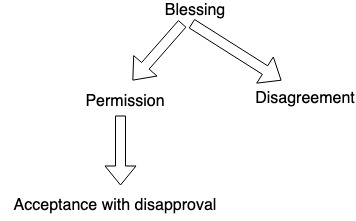
\includegraphics[width=3.0957in,height=1.922in,width=\textwidth]{mikhailov-img001.jpg}

\end{center}
\begin{styleStandard}
Although \textit{bog} ‘god’ occupies the first row of Table 2 and is almost twice as frequent as \textit{č\textcyrillic{ёrt}} ‘devil’, the words with negative connotations clearly dominate the list, and the sums of frequencies of the expressions with the negatively coloured headwords outmatch the positively coloured. The result is 17,369 versus 12,650, which makes 58\% against 42\%. Even in cases where the headword is positively coloured, there might be contexts with negative connotations (e.g. example (5)).
\end{styleStandard}

\begin{styleStandard}
To sum up, the meanings of the construction are interrelated and have many borderline cases. For this reason, it is practical not to treat them as separate homonymous constructions, but rather as a single construction.
\end{styleStandard}


\setcounter{listWWNumvleveli}{0}
\begin{listWWNumvleveli}
\item 
\begin{stylelsSectioni}
Constructing the construction
\end{stylelsSectioni}
\end{listWWNumvleveli}
\begin{styleStandard}
To present the \textit{N-s-N} construction as a whole, I will take advantage of the box notation used in Construction Grammar (CxG). This notation is “a convenient way of organizing all the information needed to give an adequate account of linguistic structure” (Fried \& Östman 2004: 13). The result of summing up the findings from the concordances is presented in the following box diagrams (Fig. 2–4).
\end{styleStandard}

\begin{styleStandard}
In section 3, the existence of semantic and structural variation in the research data was demonstrated. The easiest way to handle this heterogeneity is to define three variants of the construction \textit{N-s-N}. Still, it is better to treat them as variants of the same construction rather than as independent constructions. The first variant (\textit{N-s-N\_a}, Fig. 2) covers the meaning ‘blessing’; the second one (\textit{N-s-N\_b}, Fig. 3) has the meaning ‘disagreement’, ‘surprise’, or ‘disbelief’; and the last one (\textit{N-s-N\_c}, Fig. 4) handles the remaining meanings.
\end{styleStandard}

\begin{styleStandard}
The construction \textit{N-s-N\_a} (Fig. 2) is the simplest. The choice of the first noun is limited to three: \textit{bog} ‘god’, \textit{gospod’} ‘Lord’, and \textit{Hristos} ‘Christ’. The second nominal component is always a second-person pronoun. This pronoun can be explicitated by the optional noun phrase with the noun in the Nominative (or, rather, Vocative) case. The beneficiary of this construction is always a person (or a personified animal/artefact, etc).
\end{styleStandard}

\begin{flushleft}
\tablefirsthead{}
\tablehead{}
\tabletail{}
\tablelasttail{}
\begin{supertabular}{m{4.6233597in}}
\begin{center}
 [Warning: Image ignored] % Unhandled or unsupported graphics:
%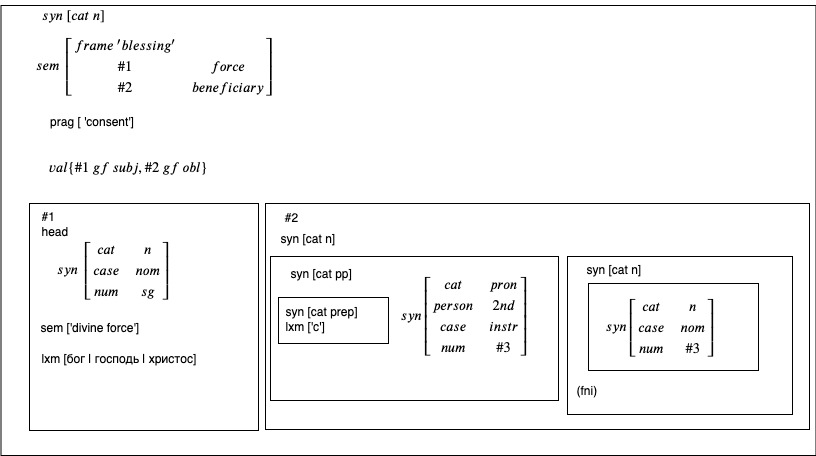
\includegraphics[width=4.248in,height=2.3736in,width=\textwidth]{mikhailov-img002.jpg}

\end{center}
\\
{\fontsize{10pt}{12.0pt}\selectfont\itshape Fig. 2. The representation of the N-s-N\_a construction.}\\
\end{supertabular}
\end{flushleft}

\setcounter{listWWNumiileveli}{0}
\begin{listWWNumiileveli}
\item 

\setcounter{listWWNumiilevelii}{0}
\begin{listWWNumiilevelii}
\item 
\begin{stylelsSourceline}
\textcyrillic{Здоровья Вам и Вашим близким, терпения! }\textcyrillic{Бог с Вами!}
\end{stylelsSourceline}
\end{listWWNumiilevelii}
\end{listWWNumiileveli}
\begin{stylelsIMT}
health.N\_Gen you.Pron\_2p\_Dat\_Pl and.Conj you.Pron\_Poss\_Dat\_Pl relative.N\_Dat\_Pl, patience.N\_Gen! God.N\_Nom with.Prep you\_2p\_Instr\_Pl
\end{stylelsIMT}

\begin{stylelsTranslation}
“I wish you and your relatives health and patience. God be with you!”
\end{stylelsTranslation}

\begin{listWWNumiileveli}
\item 
\begin{listWWNumiilevelii}
\item 
\begin{stylelsSourceline}
\textcyrillic{Прощай, Оля, господь с тобой.}
\end{stylelsSourceline}
\end{listWWNumiilevelii}
\end{listWWNumiileveli}
\begin{stylelsIMT}
farewell.Adv Olja.N\_Proper\_Nom, Lord.N\_Nom with.Prep you.Pron\_2p\_Instr\_Sg
\end{stylelsIMT}

\begin{stylelsTranslation}
“Farewell Olja, the Lord be with you.”
\end{stylelsTranslation}

\begin{listWWNumiileveli}
\item 
\begin{listWWNumiilevelii}
\item 
\begin{stylelsSourceline}
\textcyrillic{Прощайте! Христос с вами!}
\end{stylelsSourceline}
\end{listWWNumiilevelii}
\end{listWWNumiileveli}
\begin{stylelsIMT}
farewell.Adv! Christ.N\_Nom with.Prep you.Pron\_2p\_Instr\_Pl
\end{stylelsIMT}

\begin{stylelsTranslation}
“Farewell! Christ be with you!”
\end{stylelsTranslation}

\begin{styleStandard}
The variant \textit{N-s-N\_b} (Fig. 3) looks very similar to the previous one and can be easily confused with it, as we will see in section 5 of this chapter. When spoken, the intonation of this variant is different from \textit{N-s-N\_a}, with a phrasal stress on the first nominal element; graphically it may be expressed with the exclamation mark. Besides, there is a structural difference: an optional particle \textit{nu} or \textit{da} in the beginning.
\end{styleStandard}

\begin{flushleft}
\tablefirsthead{}
\tablehead{}
\tabletail{}
\tablelasttail{}
\begin{supertabular}{m{4.7427597in}}
\begin{center}
 [Warning: Image ignored] % Unhandled or unsupported graphics:
%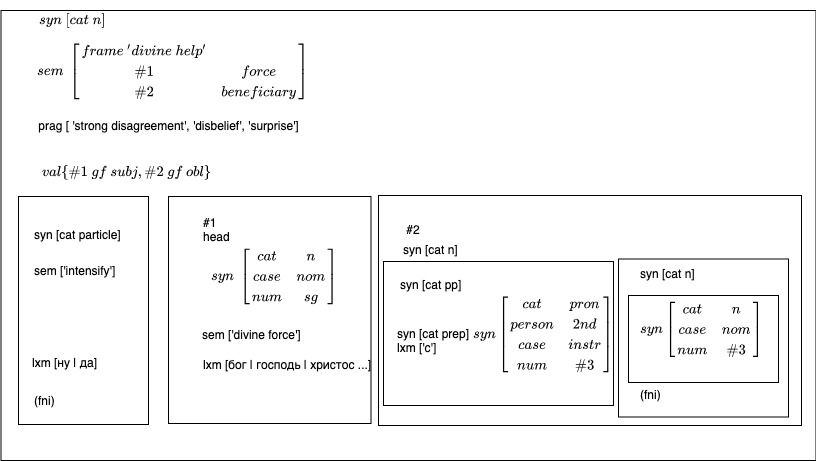
\includegraphics[width=4.6717in,height=2.639in,width=\textwidth]{mikhailov-img003.jpg}

\end{center}
\\
{\fontsize{10pt}{12.0pt}\selectfont\itshape Fig. 3. The representation of the N-s-N\_b construction.}\\
\end{supertabular}
\end{flushleft}
\begin{listWWNumiileveli}
\item 
\begin{listWWNumiilevelii}
\item 
\begin{stylelsSourceline}
\textcyrillic{Я ведь тебя убить хотел... – Что ты, Бог с тобой!}
\end{stylelsSourceline}
\end{listWWNumiilevelii}
\end{listWWNumiileveli}
\begin{stylelsIMT}
I.Pron\_1p\_Nom\_Sg but.Particle you.Pron\_2p\_Acc\_Sg kill.V\_Inf want.V\_Past\_m\_Sg. what.Pron you.Pron\_2p\_Nom\_Sg. god.N\_Nom with.Prep you.Pron\_2p\_Instr\_Sg!
\end{stylelsIMT}

\begin{stylelsTranslation}
“I wanted to kill you… – What are you talking about? I don’t believe you.”
\end{stylelsTranslation}

\begin{listWWNumiileveli}
\item 
\begin{listWWNumiilevelii}
\item 
\begin{stylelsSourceline}
\textcyrillic{Откуда это вы взяли, что я отрицаю ваше существование. }\textcyrillic{Да Бог с вами!}
\end{stylelsSourceline}
\end{listWWNumiilevelii}
\end{listWWNumiileveli}
\begin{stylelsIMT}
where.Pron this.Pron you.Pron\_2p\_Nom\_Pl. take.Past\_Pl that.Pron I.Pron\_1p\_Nom\_Sg negate.V\_Pres\_1p\_Sg you.Pron\_2p\_Poss\_Acc\_Sg existence.N\_Acc\_Sg. and.Particle god.N\_Nom with.Prep you.Pron\_2p\_Instr\_Pl
\end{stylelsIMT}

\begin{stylelsTranslation}
“How did you decide that I do not believe in your existence? This is not true!”
\end{stylelsTranslation}

\begin{listWWNumiileveli}
\item 
\begin{listWWNumiilevelii}
\item 
\begin{stylelsSourceline}
… \textcyrillic{говорят, что повально вся молодежь идет в вузы. Да господь с вами.}
\end{stylelsSourceline}
\end{listWWNumiilevelii}
\end{listWWNumiileveli}
\begin{stylelsIMT}
… say.V\_Pres\_3p\_Pl that\_Pron “in mass”.Adv all.Pron\_f\_Nom\_Sg ”young people”.N\_Nom\_Sg go.V\_Pres\_3p\_Sg to.Prep university.N\_Acc\_Pl. and.Particle Lord.N\_Nom with.Prep you.Pron\_2p\_Instr\_Pl
\end{stylelsIMT}

\begin{stylelsTranslation}
“They say all young people go to universities. No way!”
\end{stylelsTranslation}

\begin{listWWNumiileveli}
\item 
\begin{listWWNumiilevelii}
\item 
\begin{stylelsSourceline}
\textcyrillic{Лапшинов с нарочитым негодованием успокаивал: - Что ты, Никита! }\textcyrillic{Христос с тобой!}
\end{stylelsSourceline}
\end{listWWNumiilevelii}
\end{listWWNumiileveli}
\begin{stylelsIMT}
Lapshinov.N\_Proper\_Nom with.Prep faked.Adj\_Instr\_Sg indignation.N\_Instr\_Sg pacify.V\_Past\_m\_Sg. what.Pron you.Pron\_2p\_Sg, Nikita.N\_Proper\_Nom! Christ.N\_Nom with.Prep you.Pron\_2p\_Instr\_Sg
\end{stylelsIMT}

\begin{stylelsTranslation}
“Lapshinov was pacifying him with a faked indignation. Nikita, what are you (doing/saying)? You don’t mean it!”
\end{stylelsTranslation}

\begin{flushleft}
\tablefirsthead{}
\tablehead{}
\tabletail{}
\tablelasttail{}
\begin{supertabular}{m{4.7427597in}}
\begin{center}
 [Warning: Image ignored] % Unhandled or unsupported graphics:
%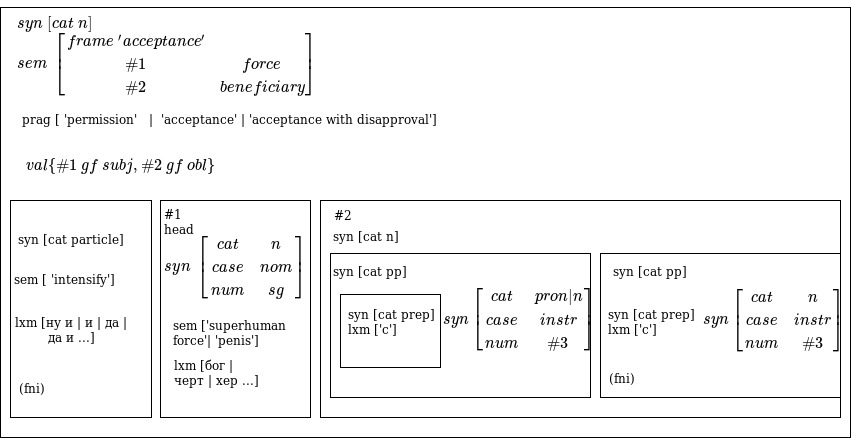
\includegraphics[width=4.4602in,height=2.2953in,width=\textwidth]{mikhailov-img004.jpg}

\end{center}
\\
{\fontsize{10pt}{12.0pt}\selectfont\itshape Fig. 4. The representation of the N-s-N\_\textcyrillic{с construction.}}\\
\end{supertabular}
\end{flushleft}
\begin{styleStandard}
The construction \textit{N-s-N\_\textcyrillic{с}} (Fig. 4) gives more freedom to choose the first nominal element. Any noun from the list of Table 2 can be used, including the three nouns used in the \textit{N-s-N\_a} and \textit{N-s-N\_b} variants, and the list is open and other nouns with the semantics of ‘superhuman force’ can be used (see section 3 for details). The second nominal element can be a noun or a pronoun, and there are no semantic restrictions: it can be a person, a thing, an activity, a situation, etc.
\end{styleStandard}

\begin{styleStandard}
This variant can have an optional initial element: a particle or a combination of particles that work as an intensifier. The palette is richer than in \textit{N-s-N\_b}, which has only two options. At least the following combinations are used quite frequently: \textit{da, i},\textit{ da i},\textit{ nu i}, and\textit{ nu da i}. The most frequently used is the combination \textit{nu i} (3,582 examples in the concordance). The expression \textit{nu i} is used in other contexts as well (e.g. \textit{Nu i durak} ‘what a fool you are’), and Dobrovol’skij et al. 2019 claim that it is a separate construction.
\end{styleStandard}

\begin{listWWNumiileveli}
\item 
\begin{listWWNumiilevelii}
\item 
\begin{stylelsSourceline}
\textcyrillic{Диска с ПО, естественно, тоже никакого нет, ну и аллах с ним.}
\end{stylelsSourceline}
\end{listWWNumiilevelii}
\end{listWWNumiileveli}
\begin{stylelsIMT}
disk.N\_Gen\_Sg with.Prep software.N\_Abr, ”of course”.Adv, also.Particle none.Pron\_Gen\_Sg no.Pred, well.Particle and.Particle Allah.N\_Nom with.Prep he.Pron\_3p\_Instr\_Sg
\end{stylelsIMT}

\begin{stylelsTranslation}
“Of course there is no software included, well, I don’t care.”
\end{stylelsTranslation}

\begin{listWWNumiileveli}
\item 
\begin{listWWNumiilevelii}
\item 
\begin{stylelsSourceline}
\textcyrillic{Да бес с ними, с британцами.}
\end{stylelsSourceline}
\end{listWWNumiilevelii}
\end{listWWNumiileveli}
\begin{stylelsIMT}
and.Particle devil.N\_Nom.N\_Nom\_Sg with.Prep he.Pron\_Instr\_3p\_Pl with.Prep brit.N\_Instr\_Pl
\end{stylelsIMT}

\begin{stylelsTranslation}
“I don’t care about the brits.”
\end{stylelsTranslation}

\begin{listWWNumiileveli}
\item 
\begin{listWWNumiilevelii}
\item 
\begin{stylelsSourceline}
\textcyrillic{Радуйтесь, и Господь с вами.}
\end{stylelsSourceline}
\end{listWWNumiilevelii}
\end{listWWNumiileveli}
\begin{stylelsIMT}
enjoy.V\_Imper\_Pl and.Particle Lord.N\_Nom with.Prep you.Pron\_2p\_Instr\_Pl
\end{stylelsIMT}

\begin{stylelsTranslation}
“Be happy and the Lord be with you.”
\end{stylelsTranslation}

\begin{styleStandard}
Another optional component is the prepositional phrase, which can be used for the explicitation of the second nominal element if the latter is a pronoun. Unlike the construction N-s-N\_a, this element is not in the Nominative case, but it repeats the structure of the second element: preposition s ‘with’ + noun phrase in the Instrumental case.
\end{styleStandard}

\begin{styleStandard}
This prepositional phrase can be a combination of a preposition with a single noun (9a), but it can have quite a complicated structure (9b and 9c).
\end{styleStandard}

\begin{listWWNumiileveli}
\item 
\begin{listWWNumiilevelii}
\item 
\begin{stylelsSourceline}
\textcyrillic{Черт с ним, с народом!}
\end{stylelsSourceline}
\end{listWWNumiilevelii}
\end{listWWNumiileveli}
\begin{stylelsIMT}
devil.N\_Nom with.Prep he.Pron\_Instr\_Sg, with.Prep people.Pron\_Instr\_Sg
\end{stylelsIMT}

\begin{stylelsTranslation}
“I don’t care about the people!”
\end{stylelsTranslation}

\begin{listWWNumiileveli}
\item 
\begin{listWWNumiilevelii}
\item 
\begin{stylelsSourceline}
\textcyrillic{Бог с ней, с этой конкретной передачей.}
\end{stylelsSourceline}
\end{listWWNumiilevelii}
\end{listWWNumiileveli}
\begin{stylelsIMT}
god.N\_Nom with.Prep she.Pron\_3p\_f\_Instr\_Sg with.Prep this.Pron\_Instr\_Sg concrete.Adj\_Instr\_Sg programme.N\_f\_Instr\_Sg
\end{stylelsIMT}

\begin{stylelsTranslation}
“I don’t care about this particular programme.”
\end{stylelsTranslation}

\begin{listWWNumiileveli}
\item 
\begin{listWWNumiilevelii}
\item 
\begin{stylelsSourceline}
\textcyrillic{Впрочем, аллах с ними, с нашими смешными читательскими проблемами!}
\end{stylelsSourceline}
\end{listWWNumiilevelii}
\end{listWWNumiileveli}
\begin{stylelsIMT}
anyway.Adv, Allah.N\_Nom with.Prep it.Pron\_Instr\_3p\_Pl with.Prep our.Pron\_Poss\_Instr\_Pl funny.Adj\_Instr\_Pl reader.Adj\_Instr\_Pl problem.N\_f\_Instr\_Pl
\end{stylelsIMT}

\begin{stylelsTranslation}
“Anyway I do not care about our funny readers’ problems!”
\end{stylelsTranslation}

\begin{styleStandard}
In rare cases, the use of two pronouns is possible, like in (10), where the speaker is the beneficiary.
\end{styleStandard}

\begin{listWWNumiileveli}
\item 
\end{listWWNumiileveli}
\begin{stylelsSourceline}
\textcyrillic{Бог с ним, со мной.}
\end{stylelsSourceline}

\begin{stylelsIMT}
god.N\_Nom with.Prep he.Pron\_3p\_m\_Instr\_Sg with.Prep I.Pron\_1p\_Instr\_Sg
\end{stylelsIMT}

\begin{stylelsTranslation}
“I do not care about myself.”
\end{stylelsTranslation}

\begin{styleStandard}
If the context is limited, the construction may become ambiguous, as in example (11), which can be interpreted as a blessing, as an acceptance, and even as disagreement.
\end{styleStandard}

\begin{listWWNumiileveli}
\item 
\end{listWWNumiileveli}
\begin{stylelsSourceline}
– \textcyrillic{Друже Чумак, {\textless}…{\textgreater} я не требую никаких объяснений. Бог с вами.}
\end{stylelsSourceline}

\begin{stylelsIMT}
friend.N\_Voc Chumak.N\_Proper\_Nom I.Pron\_Nom\_Sg no.Particle demand.V\_Pres\_1p\_Sg no.Pron\_Neg\_Gen\_Pl explanation.N\_Gen\_Pl. god.N\_Nom with.Prep you.Pron\_Instr\_Pl
\end{stylelsIMT}

\begin{stylelsTranslation}
“Friend Chumak, I am not demanding any explanations. God be with you / I do not care / Not at all.”
\end{stylelsTranslation}

\begin{styleStandard}
The most frequently used is the construction N-s-N\_c. A check of the same random sample of 1,000 examples that was used for calculating the precision of the search (see section 2) confirmed this: among the 991 correct examples, only 49 (4.9\%) belonged to N-s-N\_a. The construction N-s-N\_b occurred about the same number of times, in 47 examples (4.7\%), and all the remaining 895 (90.3\%) examples belonged to N-s-N\_c.
\end{styleStandard}


\setcounter{listWWNumvleveli}{0}
\begin{listWWNumvleveli}
\item 
\begin{stylelsSectioni}
The challenges of parallel concordancing
\end{stylelsSectioni}
\end{listWWNumvleveli}
\begin{styleStandard}
To check the equivalents that are used when translating contexts containing a certain construction, one needs many examples from parallel texts. This becomes a problem when studying multiword expressions, because their frequencies are low and therefore large amounts of text are needed to get enough examples. As it has already been mentioned, the best source of data for studying idiomatic expressions are fiction and mass media texts. Such texts are available in parallel corpora, but the sizes of parallel corpora of literary texts are quite modest compared to gigaword monolingual corpora. The data I used for this study were as follows:
\end{styleStandard}


\setcounter{listWWNumivleveli}{0}
\begin{listWWNumivleveli}
\item 
\begin{stylelsEnumerated}
Parallel corpora at the Russian National Corpus (RNC)
\end{stylelsEnumerated}
\end{listWWNumivleveli}
\begin{listWWNumiiileveli}
\item 
\begin{stylelsBulletList}
Russian-English subcorpus (6.5 M running words)
\end{stylelsBulletList}
\item 
\begin{stylelsBulletList}
English-Russian subcorpus (18 M running words)
\end{stylelsBulletList}
\end{listWWNumiiileveli}

\setcounter{listWWNumivleveli}{0}
\begin{listWWNumivleveli}
\item 
\begin{stylelsEnumerated}
Parallel corpora at Tampere University
\end{stylelsEnumerated}
\end{listWWNumivleveli}
\begin{listWWNumiiileveli}
\item 
\begin{stylelsBulletList}
ParRus, the Russian-Finnish corpus of fiction texts (6 M running words)
\end{stylelsBulletList}
\item 
\begin{stylelsBulletList}
ParFin, the Finnish-Russian corpus of fiction texts (3 M running words)
\end{stylelsBulletList}
\end{listWWNumiiileveli}
\begin{styleStandard}
It is obvious that the amounts of data from these parallel corpora are microscopic in comparison with ruTenTen11. Besides, the Russian-English subcorpus of the RNC is not well-balanced: works by Vladimir Nabokov clearly dominate over all other authors and periods. However, there were no other data available. Parallel corpora at SketchEngine are larger, but their composition is unclear, and it is impossible to filter out indirect translations and pseudotranslations. Hence, our data will be suitable only for detecting general tendencies for some of the expressions.
\end{styleStandard}

\begin{flushleft}
\tablefirsthead{}
\tablehead{}
\tabletail{}
\tablelasttail{}
\begin{supertabular}{|m{0.5656598in}|m{0.42955986in}|m{0.7768598in}|m{0.35805985in}|m{0.27335986in}|m{0.35805985in}|m{0.27335986in}|m{0.31365985in}|m{0.35385984in}|m{0.31365985in}|m{0.27335986in}|}
\hline
{\mdseries Word} &
 &
 &
{\mdseries RuEn F} &
{\mdseries ipm} &
{\mdseries EnRu F} &
{\mdseries ipm} &
{\mdseries RuFi F} &
{\mdseries ipm} &
{\mdseries FiRu F} &
{\mdseries ipm}\\\hline
{\mdseries \textcyrillic{бог}} &
{\mdseries bog} &
{\mdseries ‘god’} &
{\mdseries 65} &
{\mdseries 9.86} &
{\mdseries 23} &
{\mdseries 1.27} &
{\mdseries 73} &
{\mdseries 23.09} &
{\mdseries 9} &
{\mdseries 5.03}\\\hline
{\mdseries \textcyrillic{господь}} &
{\mdseries gospod[2B9?]} &
{\mdseries ‘Lord’} &
{\mdseries 8} &
{\mdseries 1.21} &
{\mdseries 13} &
{\mdseries 0.72} &
{\mdseries 0} &
{\mdseries 0} &
{\mdseries 0} &
{\mdseries 0}\\\hline
{\mdseries \textcyrillic{пес}} &
{\mdseries pes} &
{\mdseries ‘dog’} &
{\mdseries 1} &
{\mdseries 0.15} &
{\mdseries 0} &
{\mdseries 0} &
{\mdseries 0} &
{\mdseries 0} &
{\mdseries 0} &
{\mdseries 0}\\\hline
{\mdseries \textcyrillic{Христос}} &
{\mdseries Hristos} &
{\mdseries ‘Christ’} &
{\mdseries 10} &
{\mdseries 1.52} &
{\mdseries 0} &
{\mdseries 0} &
{\mdseries 0} &
{\mdseries 0} &
{\mdseries 0} &
{\mdseries 0}\\\hline
{\mdseries \textcyrillic{черт}} &
{\mdseries čert} &
{\mdseries ‘devil’} &
{\mdseries 42} &
{\mdseries 6.37} &
{\mdseries 28} &
{\mdseries 1.55} &
{\mdseries 52} &
{\mdseries 16.44} &
{\mdseries 6} &
{\mdseries 3.35}\\\hline
{\mdseries \textcyrillic{шут}} &
{\mdseries šut} &
{\mdseries ‘clown’} &
{\mdseries 2} &
{\mdseries 0.30} &
{\mdseries 1} &
{\mdseries 0.06} &
{\mdseries 0} &
{\mdseries 0} &
{\mdseries 0} &
{\mdseries 0}\\\hline
{\mdseries \textcyrillic{хрен}} &
{\mdseries hren} &
{\mdseries ‘horseradish’} &
{\mdseries 0} &
{\mdseries 0} &
{\mdseries 9} &
{\mdseries 0.50} &
{\mdseries 0} &
{\mdseries 0} &
{\mdseries 0} &
{\mdseries 0}\\\hline
\end{supertabular}
\end{flushleft}
\begin{stylecaption}
Table 3. Frequencies of the headwords N-s-N construction in the parallel corpora.
\end{stylecaption}

\begin{styleStandard}
It is easy to observe in Table 3 that the normalized frequencies of headwords are much higher than in ruTenTen11, although not all expressions were found (only seven of fifteen). This can be explained by the structure of ruTenTen11, which contains many genres in which the construction \textit{N-s-N} is never used. The causes of the differences in frequencies between parallel corpora are the corpora’s imbalance and their construction from whole texts, so a couple of very long texts could skew the whole collection.
\end{styleStandard}

\begin{styleStandard}
The comparison of the frequencies of \textit{N-s-N} in ruTenTen11 and the parallel corpora demonstrates that the frequencies of expressions are much less stable than that of single words, and it is problematic to obtain reliable statistics from the observations. For example, the frequency of the expression \textit{bog s X} is 9.8 ipm in Russian-English RNC and 23.1 ipm in ParRus, although both corpora are collections of Russian fiction texts.
\end{styleStandard}

\begin{styleStandard}
Regardless, one important observation can be made from the frequencies: the construction \textit{N-s-N} is much more frequent in the original Russian texts than in the translations from English and Finnish into Russian. This is the sign of the evident absence of matching constructions in both English and Finnish. The findings are also in line with Tirkkonen-Condit’s (2004) hypothesis about the underrepresentation of unique items of the source language in translated language.
\end{styleStandard}

\begin{styleStandard}
The statistics from the parallel concordances give the impression that something is not right. As it was shown in the previous sections, the construction \textit{N-s-N} is polysemous, and the actual meaning depends on the context. The most misleading is the construction with \textit{bog} ‘god’ as a headword: it can be used in all three variants of the construction described in section 4 of this paper. The variant \textit{N-s-N\_a} is not very frequent: I demonstrated this by the study of random examples. Still, in the Russian-English data, 28 contexts out of 65 were translated into English with expressions containing the word \textit{god}. In the Russian-Finnish data, there are 73 contexts with \textit{bog} ‘god’, and 48 of them are translated with the expressions containing \textit{jumala} ‘god’, \textit{herra} ‘Lord’, or \textit{luoja} ‘Creator’. From the above-mentioned study of random examples, I would have expected that only about 7\% of contexts of \textit{bog s X} would belong to the \textit{N-s-N\_a} variant, while the statistics from the parallel corpora show a much higher rate in both the Russian-English and Russian-Finnish data.
\end{styleStandard}

\begin{styleStandard}
It is true that the data are not balanced, and it is true that the frequencies of the expressions in our data vary greatly. It is therefore quite possible that the data from the parallel corpora might contain far more \textit{N-s-N\_a} contexts than the ruTenTen11 data. For this reason, it is necessary to check the actual contexts to confirm the statistical observations.
\end{styleStandard}

\begin{styleStandard}
The checking of the Russian-English concordance with \textit{bog} ‘god’ on the Russian side and \textit{god} on the English side confirmed my suspicions: 19 cases out of 28 show an obvious misunderstanding of the source text.
\end{styleStandard}


\setcounter{listWWNumiileveli}{0}
\begin{listWWNumiileveli}
\item 
\end{listWWNumiileveli}
\begin{stylelsSourceline}
« \textcyrillic{Ну, бог с тобой, оставайся уж», — решила в тоске Грушенька, сострадательно ему улыбнувшись.}
\end{stylelsSourceline}

\begin{stylelsIMT}
“well.Particle god.N\_Nom with.Prep you.Pron\_2p\_Instr\_Sg stay.V\_Imper well.Particle”, - decide.V\_Past\_f\_Sg in.Prep melancholy.N\_Loc\_Sg Grushenka.N\_Proper\_Nom, compassionately.Adv he.Pron\_Dat\_Sg smile.V\_Gerund
\end{stylelsIMT}

\begin{stylelsTranslation}
“OK, I don’t care, you can stay, decided Grushenka in her melancholy and smiled at him compassionately.”
\end{stylelsTranslation}

\begin{stylelsSourceline}
“Well, God bless you, you’d better stay, then,” Grushenka decided in her grief, smiling compassionately at him.
\end{stylelsSourceline}

\begin{stylelsTranslation}
F. Dostoevsky. Brat[2B9?]â Karamazovy [The Brothers Karamazov] (1878, transl. C. Garnett, 1912)
\end{stylelsTranslation}

\begin{styleStandard}
In example (12), the speaker reluctantly gives the interlocutor her permission to stay, while the translator obviously understood the expression as a blessing or at least as a demonstration of piety (which is strange for Grushenka, who, as we know, was not a very pious person).
\end{styleStandard}

\begin{styleStandard}
In the Russian-Finnish data, 44 contexts with an obvious misunderstanding were found. An additional factor for misinterpreting is Russian-Finnish dictionaries, some of which register the phrase \textit{bog s X} only with the meaning of blessing (see, e.g. Kuusinen \& Ollikainen 1984).
\end{styleStandard}

\begin{listWWNumiileveli}
\item 
\end{listWWNumiileveli}
\begin{stylelsSourceline}
\textcyrillic{Господин Разумихин не то-с, да и человек посторонний, прибежал ко мне весь такой бледный ... Ну да бог с ним, что его сюда мешать.}
\end{stylelsSourceline}

\begin{stylelsIMT}
mister.N\_Nom\_Sg Razumihin.N\_Proper\_Nom not.Particle that.Pron, and.Particle and.Patricle person.N\_Nom\_Sg stranger.Adj\_Nom\_m\_Sg, run.V\_Past\_m\_Sg to.Prep I.Pron\_1p\_Dat all.Pron\_m\_Nom such.Adj\_Nom\_Sg pale.Adj\_Nom\_m\_Sg. but.Particle and.Particle god.N\_m\_Nom with.Prep he.Pron\_3p\_Instr\_Sg, what.Pron he.Pron\_3p\_Acc\_Sg here.Adv involve.V\_Inf
\end{stylelsIMT}

\begin{stylelsTranslation}
“Mister Razumihin is a stranger, but he ran to me so pale. Never mind, why shall we involve him in this.”
\end{stylelsTranslation}

\begin{stylelsSourceline}
Herra Razumihinhan on vallan toista maata, sivullinen ihminen, vaikka hän juoksi silloin kasvot kalpeina luokseni ... Luoja hänen kanssaan, eihän hänellä ole tässä osaa eikä arpaa.
\end{stylelsSourceline}

\begin{stylelsIMT}
mister.N\_Nom Razumihin.N\_Nom be.V\_Pres power.N\_Gen another.Adj\_Partitive country.N\_Partitive stranger.Adj\_Nom person.N\_Nom although.Conj he.Pron\_Nom run.V\_Past then.Adv face.N\_Nom white.Adj\_Essive ”to me”.Adv. Lord.N\_Nom he.Pron\_Gen with.Postposition not.Particle he.Pron\_3p\_Allative be.V\_Pres here.Adv\_Adessive part.N\_Partitive not.Particle lot.N\_Partitive\_Sg
\end{stylelsIMT}

\begin{stylelsTranslation}
“Mister Razumihin is like from another country, a stranger, still he ran to me with a white face. God be with him, he has nothing to do in this business.”
\end{stylelsTranslation}

\begin{stylelsTranslation}
F. Dostoevsky. Prestuplenie i nakazanie [Crime and Punishment] (1866, transl. J. Konkka, 1970)
\end{stylelsTranslation}

\begin{styleStandard}
The expression \textit{č\textcyrillic{ёrt s X}} ‘devil with X’ also contains a trap: it can be interpreted as swearing and blasphemy, although in most cases it does not and fits quite well into the \textit{N-s-N\_c} construction.
\end{styleStandard}

\begin{listWWNumiileveli}
\item 
\end{listWWNumiileveli}
\begin{stylelsSourceline}
\textcyrillic{Об чем? Ну, да черт с тобой, пожалуй, не сказывай.}
\end{stylelsSourceline}

\begin{stylelsIMT}
about.Prep what.Pron\_Loc well.Particle and.Particle devil.N\_Nom with.Prep you.Pron\_Instr\_Sg maybe.Adv not.Particle tell.V\_Imper\_Sg
\end{stylelsIMT}

\begin{stylelsTranslation}
“What about? Well, do not tell, I don’t mind.”
\end{stylelsTranslation}

\begin{stylelsSourceline}
What about? Confound you, don’t tell me then.
\end{stylelsSourceline}

\begin{stylelsTranslation}
F. Dostoevsky. Prestuplenie i nakazanie [Crime and Punishment] (1866, transl. C. Garnett, 1914)
\end{stylelsTranslation}

\begin{styleStandard}
One might think that such things take place only in very old translations of even older source texts. However, this is not so: in (15) is an example of a relatively recently published translation from Russian into Finnish.
\end{styleStandard}

\begin{listWWNumiileveli}
\item 
\end{listWWNumiileveli}
\begin{stylelsSourceline}
\textcyrillic{Черт с ним! }– \textcyrillic{сердито подумала Вероника.}
\end{stylelsSourceline}

\begin{stylelsIMT}
devil.N\_Nom with.Prep he.Pron\_Instr\_Sg angrily.Adv think.V\_Past\_f\_Sg Veronika.N\_Proper\_Nom.
\end{stylelsIMT}

\begin{stylelsTranslation}
“I don’t care, thought Veronika angrily.”
\end{stylelsTranslation}

\begin{stylelsIMT}
”Hitto”, Veronika mietti vihaisena.
\end{stylelsIMT}

\begin{stylelsIMT}
devil.N\_Nom, Veronika.N\_Proper\_Nom think.V\_Past\_3p\_Sg angry.Adj\_Essive\_Sg
\end{stylelsIMT}

\begin{stylelsTranslationSubexample}
“Devil, thought Veronika angrily.”
\end{stylelsTranslationSubexample}

\begin{stylelsTranslationSubexample}
A. Marinina. Za vse nado platit[2B9?] [You have to pay for everything] (1995, transl. O. Kuukasjärvi, 2005)
\end{stylelsTranslationSubexample}

\begin{styleStandard}
It should be mentioned that the parallel concordance also provided enough examples with interesting solutions for this construction. I will give here only two examples from the Russian-English data. In (16a) an English expression \textit{all right} is used, while in (16b) the meaning of expression is explicitated (\textit{I will take it}).
\end{styleStandard}

\begin{listWWNumiileveli}
\item 
\begin{listWWNumiilevelii}
\item 
\begin{stylelsSourceline}
{}- \textcyrillic{Ну что ж, бог с вами, пусть пять рублей будет. }\textcyrillic{Только деньги попрошу вперед.}
\end{stylelsSourceline}
\end{listWWNumiilevelii}
\end{listWWNumiileveli}
\begin{stylelsIMT}
well.Particle what.Pron but.Particle, god.N\_Nom with.Prep you.Pron\_2p\_Instr\_Pl, let.Particle five.Num\_Nom rouble.N\_Gen\_Pl be.V\_Future\_3p\_Sg. only.Adv money.N\_Acc\_Pl ask.V\_Fut\_1p\_Sg forward.Adv
\end{stylelsIMT}

\begin{stylelsIMT}
“OK, let it be five roubles, but I would like to have the money in advance.”
\end{stylelsIMT}

\begin{stylelsSourceline}
“Well, all right, make it five roubles. Only I want the money in advance, please.” 
\end{stylelsSourceline}

\begin{stylelsTranslationSubexample}
Ilya Ilf, Evgeny Petrov. \textcyrillic{Двенадцать стульев (Dvenadcat\textlatin{[2B9?]} stul\textlatin{[2B9?]}ev) [The Twelve Chairs] (1927, transl. John Richardson, 1961).}
\end{stylelsTranslationSubexample}

\begin{listWWNumiileveli}
\item 
\begin{listWWNumiilevelii}
\item 
\begin{stylelsSourceline}
{}- \textcyrillic{Ну, бог с вами, --- сказал Махин, кладя на витрину купон.}
\end{stylelsSourceline}
\end{listWWNumiilevelii}
\end{listWWNumiileveli}
\begin{stylelsIMT}
well.Particle god.N\_Nom with.Prep you.Pron\_2p\_Instr\_Pl say.V\_Past Mahin.N\_Proper\_Nom, put.V\_Gerund on.Prep counter.N\_Acc\_Sg coupon.N\_Acc\_Sg
\end{stylelsIMT}

\begin{stylelsIMT}
“‘OK, I agree,’ said Mahin putting the coupon on the counter”.
\end{stylelsIMT}

\begin{stylelsSourceline}
“Well, I will take it,” said Mahin, and put the coupon on the counter.
\end{stylelsSourceline}

\begin{stylelsTranslationSubexample}
Leo Tolstoy. Fal[2B9?]šivyj kupon [The Forged Coupon] (1889-1904, transl. Louise and Aylmer Maude, 1911)
\end{stylelsTranslationSubexample}

\begin{styleStandard}
To sum up the findings from the parallel concordances, the main problem of the data obtained from translations from Russian into other languages is the possibility of misunderstanding the source texts by translators. Hence, translations from other languages into Russian quite unexpectedly become a very useful source of reference data. Translators into Russian write in their native language and their work is addressed to other native speakers of Russian. As a result, the expression that served as a stimulus for the Russian expression may be with a few reservations used as an equivalent for translating in the opposite direction. Of course, in this case there is an issue of the correct understanding of the source text in language X.
\end{styleStandard}

\begin{styleStandard}
The RNC’s English-Russian subcorpus is larger and richer than the Russian-English one. In spite of this, the construction \textit{N-s-N} features in it much less frequently (see Table 3). Still, the parallel concordance produces some interesting solutions that seem suitable for translating from Russian into English as well.
\end{styleStandard}

\begin{listWWNumiileveli}
\item 
\begin{listWWNumiilevelii}
\item 
\begin{stylelsSourceline}
I’ve been told I ought to have a salon, whatever that may be. Never mind. Go on, Badger. 
\end{stylelsSourceline}
\end{listWWNumiilevelii}
\end{listWWNumiileveli}
\begin{stylelsSourceline}
\textcyrillic{Мне частенько говорили, что мне надо бы завести салон, что бы это там ни значило. Ну, бог с ним! Продолжай, Барсук.}
\end{stylelsSourceline}

\begin{stylelsIMT}
I.Pron\_1p\_Dat\_Sg often.Adv say.V\_Past\_Pl that.Pron I.Pron\_1p\_Dat\_Sg need.Pred would.Particle start.V\_Inf salon.N\_Acc\_Sg, what.Pron would.Particle this.Pron there.Adv not.Particle mean.V\_Past. well.Particle god.N\_Nom\_Sg with.Prep he.Pron\_3p\_Instr\_Sg. continue.V\_Imper, Badger.N\_Nom.
\end{stylelsIMT}

\begin{stylelsTranslation}
“They often said to me that I should start a salon, whatever it may mean. Continue, Badger.”
\end{stylelsTranslation}

\begin{stylelsTranslationSubexample}
Kenneth Grahame. The Wind in the Willows, (1908, transl. I.~Tokmakova, 1988)
\end{stylelsTranslationSubexample}

\begin{listWWNumiileveli}
\item 
\begin{listWWNumiilevelii}
\item 
\begin{stylelsSourceline}
“You still have half your balls there.” “I don’t care. This will set my game back a month.”
\end{stylelsSourceline}
\end{listWWNumiilevelii}
\end{listWWNumiileveli}
\begin{stylelsSourceline}
– \textcyrillic{У тебя еще осталась половина мячей. }– \textcyrillic{И черт с ним. Это отбросит мою технику на месяц назад.}
\end{stylelsSourceline}

\begin{stylelsIMT}
by.Prep you.Pron\_2p\_Gen\_Sg still.Particle remain.V\_Past\_f\_Sg half.N\_Nom\_Sg ball.N\_Gen\_Pl. and.Particle devil.N\_Nom with.Prep he.Pron\_3p\_Instr\_Sg. It.Pron throw.V\_Future\_3p\_Sg my.Pron\_Poss\_f\_Acc\_Sg technique.N\_Acc\_Sg on.Prep month.N\_Acc\_Sg back.Adv
\end{stylelsIMT}

\begin{stylelsTranslation}
“You still have half of the balls. I don’t care. It will throw my technique a month back.”
\end{stylelsTranslation}

\begin{stylelsTranslation}
Michael Connelly. City Of Bones (2002, transl. D.~Vozniakevitch, 2006)
\end{stylelsTranslation}

\begin{styleStandard}
The same can be observed in the Finnish-Russian parallel concordance obtained from the ParFin corpus.
\end{styleStandard}

\begin{listWWNumiileveli}
\item 
\end{listWWNumiileveli}
\begin{stylelsSourceline}
Lukeneilla ihmisillä sellanen on ja hyvä niin.
\end{stylelsSourceline}

\begin{stylelsIMT}
study.V\_Participle\_Allative\_Pl person.N\_Allative\_Pl such.Adj\_Nom\_Sg be.V\_3p\_Pres\_Sg and.Conj good.Adj\_Nom\_Sg so.Adv
\end{stylelsIMT}

\begin{stylelsTranslationSubexample}
“Educated people have this and this is good.”
\end{stylelsTranslationSubexample}

\begin{stylelsSourceline}
\textcyrillic{У тех, кто учился, есть, и бог с ними.}
\end{stylelsSourceline}

\begin{stylelsIMT}
by.Prep he.Pron\_Gen\_Pl, who.Pron\_Nom study.V\_Past\_m\_Sg, be.V\_Pres\_3p, and.Particle god.N\_Nom with.Prep he.Pron\_Instr\_Pl.
\end{stylelsIMT}

\begin{stylelsTranslation}
“Those who studied have it and let it be”
\end{stylelsTranslation}

\begin{stylelsTranslationSubexample}
Hotakainen, Kari, Juoksuhaudantie (transl. I. Uretski)
\end{stylelsTranslationSubexample}

\begin{styleStandard}
Strangely, although the English stimuli \textit{never mind} and \textit{I don’t care}, as well as the Finnish stimulus \textit{hyvä niin} ‘OK’ can be considered as very good variants for conveying the meaning of the Russian construction \textit{N-s-N\_c}, they are not very typical for translations from Russian. The expression \textit{never mind} occurs only 7 times in the Russian-English concordance, and the verb \textit{care} only three times. In the Russian-Finnish parallel concordance, there is not a single example of \textit{hyvä niin} used as an equivalent for \textit{N-s-N}.
\end{styleStandard}


\setcounter{listWWNumvleveli}{0}
\begin{listWWNumvleveli}
\item 
\begin{stylelsSectioni}
Discussion
\end{stylelsSectioni}
\end{listWWNumvleveli}
\begin{styleStandard}
The case study performed in this paper demonstrates the usefulness of monolingual and parallel corpora for studying constructions. Corpora provide information on the variability of constructions and statistics. Monolingual concordancing is helpful in the study of the components of the construction, the lexemes used for its realization, and even semantic issues. The analysis reveals that the construction \textit{N-s-N} can be implemented in the form of ready-made phrases (like \textit{bog s nim, č\textcyrillic{ё}rt s nim}, etc.) that are used very frequently, as well as in the form of \textit{hapax legomena} constructed with the same template. As a result, some phrases may be registered in dictionaries, while occasionalisms remain both outside dictionaries due to their rarity and outside grammar descriptions due to their specificity. Evidently, the best way of describing and storing such units would be databases like FrameNet or Constructicon.
\end{styleStandard}

\begin{styleStandard}
To study the links of the construction with other languages, parallel corpora were used. However, the usability of this resource was limited. Parallel corpora did not help so much in looking up translation equivalents as one might have expected. The first reason was that the search did not return enough usage examples; one would have needed much larger data collections to obtain a parallel concordance at least comparable with the monolingual concordance from ruTenTen11. The data that were available were sufficient only for demonstrating the fact that the \textit{N-s-N} construction in Russian does not have corresponding constructions in English or Finnish, and that this absence causes difficulties for translators.
\end{styleStandard}

\begin{styleStandard}
The second reason was the rather high rate of errors in the translations. Of course, one might expect errors in any language data – this is quite natural – but in this case the errors were repeated, and their main cause was misinterpretation of the source text. On the one hand, this is a challenge to modern statistical and neural machine translation technologies, which are based on parallel corpora and use human translations for modelling MT. The developers of MT presume that there might be errors and mistakes in the data, but are they ready for errors on such a scale? On the other hand, this is a challenge to the belief that the translation of a literary work into another language is the \textit{same} story told in other words. The real data show that literary translators sometimes do not understand the source text well enough.
\end{styleStandard}

\begin{styleStandard}
Why does this happen? The first priority of a literary translator is to produce a good target text, one that meets the standards of a literary text. The correspondence of the translation to the source text comes second, and it is not likely that every passage of the translation is compared to the original text. Of course, the translation should not be very different, but how correct should it be? There is also some evidence that the literary translators’ command of the source language is not as advanced as one might expect. For example, Nikolai Chukovski, one of the leading Russian literary translators working from the 1920s to the 1960s, was very critical of his own proficiency in English (Chukovski \& Chukovski 2004), and there existed writers (and especially poets) who “translated” by editing earlier translations or literal translations produced by other people (see, e.g. Kamovnikova 2019).
\end{styleStandard}

\begin{styleStandard}
These issues make the use of parallel corpora of literary texts a specific resource. They cannot be, for example, the main source of data for bilingual dictionaries, but rather reference data for rechecking translation equivalents. Parallel corpora also demonstrate that even nowadays, proficiency in non-native languages is limited and needs to be improved. The data from parallel corpora might be of great help in finding such weak points.
\end{styleStandard}

\begin{listWWNumvleveli}
\item 
\begin{stylelsSectioni}
References
\end{stylelsSectioni}

\begin{listWWNumvlevelii}
\item 
\begin{stylelsSectionii}
Scientific publications
\end{stylelsSectionii}
\end{listWWNumvlevelii}
\end{listWWNumvleveli}
\begin{styleStandard}
Baranov, Anatolij \& Dmitrij Dobrovol[2B9?]skij. 2008. \textit{Aspekty teorii frazeologii.} [Aspects of the phraseological theory]. Moskva: Znak.
\end{styleStandard}

\begin{styleStandard}
Čukovski, Kornej; Čukovskij, Nikolaj. 2004. «My očen[2B9?] raznye literatory…» [We are very different writers]. 1921-63. \textit{Znamja \# 1.} \url{http://www.chukfamily.ru/kornei/prosa/pisma/my-ochen-raznye-literatory-ki-chukovskij-nk-chukovskij-perepiska} (Accessed 1.11.20)
\end{styleStandard}

\begin{styleStandard}
Dobrovol[2B9?]skij, Dmitrij, Mihail Kopotev and Ludmila Pöppel. 2019. Gruppa konstrukcij nu i X: semantika, pragmatika, sočetaemost[2B9?]. [The group of constructions nu i X: semantics, pragmatics, combinability]. \textit{Scando-Slavica}, 65:1, 5-25, DOI: 10.1080/00806765.2019.1586578
\end{styleStandard}

\begin{styleStandard}
Dunning, Ted. 1993. Accurate Methods for the Statistics of Surprise and Coincidence. \textit{Computational Linguistics}, 19:1, 61-74. https://www.aclweb.org/anthology/J93-1003/
\end{styleStandard}

\begin{styleStandard}
Fried, Mirjam \& Jan-Ola Östman. 2004. Construction Grammar. A thumbnail sketch. In Fried, M., \& Östman, J. (eds). 2004. \textit{Construction Grammar in a Cross-Language Perspective.} Amsterdam/Philadelphia: John Benjamins, 11-86.
\end{styleStandard}

\begin{styleStandard}
Härme, Juho and Mikhail Mikhailov. 2016. From Russian to Finnish and back: compiling Russian–Finnish–Russian parallel corpora. In: Medvecká, Lubica \ (ed.) \textit{Translation from / into languages of limited diffusion 3}, 139–147. Bratislava: The Slovak society of Translators of Scientific and Technical literature.
\end{styleStandard}

\begin{styleStandard}
Kamovnikova, Natalia. 2019. \textit{Made Under Pressure: Literary Translation in the Soviet Union, 1960-1991} (Studies in Print Culture and the History of the Book). Amherst, Massachussets: University of Massachusetts Press.
\end{styleStandard}

\begin{styleStandard}
Kopotev, Mihail, and Lidia Pivovarova, and Daria Kormacheva. 2016. Constructional generalization over Russian collocations. \textit{Mémoires de la Société néophilologique de Helsinki, Tome C }(Collocations Cross-Linguistically), Helsinki, 121-140.
\end{styleStandard}

\begin{styleStandard}
Kormacheva, Daria. 2020. \textit{Collocations on the way: How words come together in Russian}. Ph. D. dissertation. Helsinki: University of Helsinki. http://urn.fi/URN:ISBN:978-951-51-6083-6
\end{styleStandard}

\begin{styleStandard}
Levshina, Natalia. 2015. \textit{How to Do Linguistics with R[202F?]: Data Exploration and Statistical Analysis.} Amsterdam: John Benjamins.
\end{styleStandard}

\begin{styleStandard}
Mikhailov Mikhail, and Juho Härme. 2015. Parallelnyje korpusa hudožestvennyh tekstov v Tamperskom universitete. [Parallel corpora of fiction texts at the University of Tampere]. \textit{Russkij jazyk za rubežom}. Spetsvypusk, 16-19.
\end{styleStandard}

\begin{styleStandard}
Nivre, Joakim and Chiao-Ting Fang. 2017. Universal Dependency Evaluation. In \textit{Proceedings of the NoDaLiDa 2017. Workshop on Universal Dependencies} (UDW 2017), 86–95, Gothenburg.
\end{styleStandard}

\begin{styleStandard}
Shavrina, Tatiana and Olga Shapovalova. 2017. To the methodology of corpus construction for machine learning: “Taiga” syntax tree corpus and parser. In \textit{Trudy meždunarodnoj konferencii “Korpusnaja lingvistika–2017”}. Sankt-Peterburg: SPbGU and ILI, 78.
\end{styleStandard}

\begin{styleStandard}
Tirkkonen-Condit, Sonja. 2004. Unique items – over or underrepresented in translated language? In Anna Mauranen and Pekka Kujamäki (eds).\textit{ Translation Universals: do they exist?} Amsterdam/Philadelphia: John Benjamins, 177-184.
\end{styleStandard}

\begin{styleStandard}
Zaharov N. V. 2008. Anglijskij âzyk v tezauruse Puškina. [The English language in the Pushkin’s thesaurus]. \textit{Znanie. Ponimanie. Umenie}. № 9. (\url{http://www.zpu-journal.ru/e-zpu/2008/9/Zakharov_English/}) (Accessed 1.11.20)
\end{styleStandard}

\begin{styleStandard}
Wierzbicka, Anna. 1987. Boys will be boys: ‘Radical semantics’ vs. ‘radical pragmatics’. \textit{Language} 63 (1): 95-114.
\end{styleStandard}

\begin{styleStandard}
Xiao, Richard 2015. Collocation. In Douglas Biber and Randy Reppen (eds). \textit{The Cambridge Handbook of English Corpus Linguistics}. Cambridge: Cambridge University Press, 106-124. https://doi.org/10.1017/CBO9781139764377
\end{styleStandard}

\begin{listWWNumvleveli}
\item 
\begin{listWWNumvlevelii}
\item 
\begin{stylelsSectionii}
Dictionaries and corpora
\end{stylelsSectionii}
\end{listWWNumvlevelii}
\end{listWWNumvleveli}
\begin{styleStandard}
Baranov, Anatolij \& Dobrovol[2B9?]skij, Dmitrij (eds) 2015. \textit{Akademičeskij slovar' russkoj frazeologii} [Academic dictionary of Russian Phraseology], LEKSRUS, Moscow.
\end{styleStandard}

\begin{styleStandard}
Constructicon for Russian. (\url{https://spraakbanken.gu.se/karp/#?mode=konstruktikon-rus}) (Accessed 1.11.20)
\end{styleStandard}

\begin{styleStandard}
enTenTen15 – English corpus from the web: (\url{https://www.sketchengine.eu/ententen-english-corpus/}) (Accessed 1.11.20)
\end{styleStandard}

\begin{styleStandard}
Kuusinen Martti, Ollikainen V. (eds.) 1984. \textit{Venäläis-Suomalainen suursanakirja} [The Large Russian-Finnish Dictionary]. WSOY, Porvoo-Helsinki-Juva.
\end{styleStandard}

\begin{styleStandard}
Ljashevskaja Olga and Sergej Sharov 2009. \textit{Častotnyj slovar[2B9?] russkogo âzyka.} (Na materialah Nacional[2B9?]nogo korpusa russkogo âzyka). [The Frequency dictionary of the Russian Language (based on Russian National Corpus)]. Moskva: Azbukovnik. http://dict.ruslang.ru. (Accessed 1.11.20)
\end{styleStandard}

\begin{styleStandard}
Lubensky, Sophia 1995. \textit{Random house Russian-English dictionary of idioms.} Random House, New York.
\end{styleStandard}

\begin{styleStandard}
MAS 1984. = Evgen[2B9?]eva A.P. (ed.) \textit{Slovar[2B9?] russkogo âzyka.} [Dictionary of Russian Language], AN SSSR, IRÂ. Moskva: Russkij âzyk.
\end{styleStandard}

\begin{styleStandard}
Ožegov S.I., Švedova N.Û. 1992. \textit{Tolkovyj slovar[2B9?] russkogo âzyka} [The Explanatory Dictionary of Russian Language]. Az[2BA?]: Moskva.
\end{styleStandard}

\begin{styleStandard}
ParRus, Finnish-Russian Parallel Corpus of Literary Texts, Tampere University, puolukka.uta.fi/texthammer (Free registration. Accessed 1.11.20)
\end{styleStandard}

\begin{styleStandard}
ParFin, Russian-Finnish Parallel Corpus of Literary Texts, Tampere University, puolukka.uta.fi/texthammer (Free registration. Accessed 1.11.20)
\end{styleStandard}

\begin{styleStandard}
Parallel corpora at the Russian National Corpus, \url{http://ruscorpora.ru/new/search-para-en.html} (Accessed 1.11.20)
\end{styleStandard}

\begin{styleStandard}
ruTenTen11 – Russian corpus from the web: \url{https://www.sketchengine.eu/rutenten-russian-corpus/} (Accessed 1.11.20)
\end{styleStandard}

\end{document}
